\documentclass[11pt]{article} 
\usepackage{amsfonts, amsmath, amssymb, amsthm,enumerate,adjustbox,mathpazo}
\usepackage[dvipsnames]{xcolor}
%colors in xcolor package are:
\usepackage{pgfplots}
\pgfplotsset{compat=1.18} 
\usepackage{tikz}
\usetikzlibrary{er,positioning,calc}
\usetikzlibrary{graphs,arrows,shapes,shadings,intersections}
%\usegdlibrary{trees}
\usetikzlibrary{decorations.markings}
\usetikzlibrary{datavisualization.formats.functions}
\usepackage[margin = 0.9in]{geometry}
\usepackage{multirow}
\usepackage{tgbonum}
\usepackage[parfill]{parskip}
\setlength{\parindent}{0pt}
\usepackage[T1]{fontenc}
\usepackage[framemethod=TikZ]{mdframed}
\mdfdefinestyle{MyFrame}{
    linecolor=black,
    outerlinewidth=1pt,
    roundcorner=5pt,
    innertopmargin=5pt,
    innerbottommargin=5pt,
    innerrightmargin=5pt,
    innerleftmargin=5pt,
    backgroundcolor=white 
}
\newcounter{higher} 
\setcounter{higher}{1}
\newcommand{\pythagwidth}{3cm}
\newcommand{\pythagheight}{2cm}
\definecolor{medgrey}{RGB}{130,130,130}
\definecolor{Acolor}{RGB}{134, 218, 200}
\newcounter{row}
\newcounter{col}
\newcommand\setrow[9]{
  \setcounter{col}{1}
  \foreach \n in {#1, #2, #3, #4, #5, #6, #7, #8, #9} {
    \edef\x{\value{col} - 0.5}
    \edef\y{9.5 - \value{row}}
    \node[anchor=center] at (\x, \y) {\n};
    \stepcounter{col}
  }
  \stepcounter{row}
}

\title{\textbf{TikZ Compilation}}
\author{Sayantani Bhattacharya}
\date{}
\begin{document}

\maketitle

\section{Calculus}
\begin{enumerate}

\item\adjustbox{valign=t}{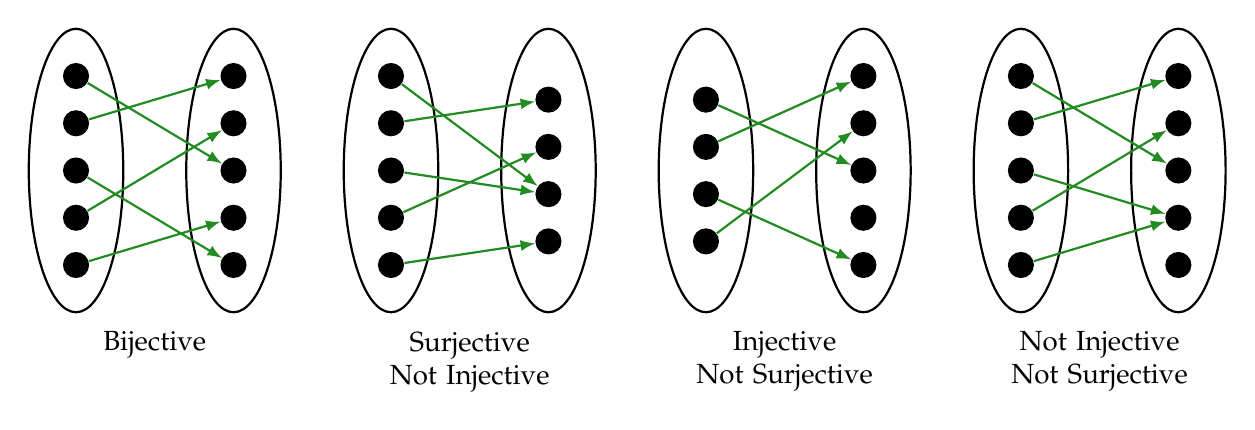
\begin{tikzpicture}[xscale=0.4,yscale=0.6] 

\begin{scope}
\draw[thick] (0,0) ellipse (1.5cm and 3cm);
\draw[thick] (5,0) ellipse (1.5cm and 3cm);

\node[fill,circle] (a1) at (0,2) {};
\node[fill,circle] (a2) at (0,1) {};
\node[fill,circle] (a3) at (0,0) {};
\node[fill,circle] (a4) at (0,-1) {};
\node[fill,circle] (a5) at (0,-2) {};

\node[fill,circle] (b1) at (5,2) {};
\node[fill,circle] (b2) at (5,1) {};
\node[fill,circle] (b3) at (5,0) {};
\node[fill,circle] (b4) at (5,-1) {};
\node[fill,circle] (b5) at (5,-2) {};

\draw[-latex,ForestGreen,thick] (a1)--(b3);
\draw[-latex,ForestGreen,thick] (a2)--(b1);
\draw[-latex,ForestGreen,thick] (a3)--(b5);
\draw[-latex,ForestGreen,thick] (a4)--(b2);
\draw[-latex,ForestGreen,thick] (a5)--(b4);

\node[below] at (2.5,-3.2) {Bijective};
\end{scope}

\begin{scope}[xshift=10cm]
\draw[thick] (0,0) ellipse (1.5cm and 3cm);
\draw[thick] (5,0) ellipse (1.5cm and 3cm);

\node[fill,circle] (a1) at (0,2) {};
\node[fill,circle] (a2) at (0,1) {};
\node[fill,circle] (a3) at (0,0) {};
\node[fill,circle] (a4) at (0,-1) {};
\node[fill,circle] (a5) at (0,-2) {};

\node[fill,circle] (b1) at (5,1.5) {};
\node[fill,circle] (b2) at (5,.5) {};
\node[fill,circle] (b3) at (5,-0.5) {};
\node[fill,circle] (b4) at (5,-1.5) {}; 

\draw[-latex,ForestGreen,thick] (a1)--(b3);
\draw[-latex,ForestGreen,thick] (a2)--(b1);
\draw[-latex,ForestGreen,thick] (a3)--(b3);
\draw[-latex,ForestGreen,thick] (a4)--(b2);
\draw[-latex,ForestGreen,thick] (a5)--(b4);

\node[below, text width=3cm, align=center] at (2.5,-3.2) {Surjective \\ Not Injective};
\end{scope}

\begin{scope}[xshift=20cm]
\draw[thick] (0,0) ellipse (1.5cm and 3cm);
\draw[thick] (5,0) ellipse (1.5cm and 3cm);

\node[fill,circle] (a1) at (0,1.5) {};
\node[fill,circle] (a2) at (0,0.5) {};
\node[fill,circle] (a3) at (0,-0.5) {};
\node[fill,circle] (a4) at (0,-1.5) {}; 

\node[fill,circle] (b1) at (5,2) {};
\node[fill,circle] (b2) at (5,1) {};
\node[fill,circle] (b3) at (5,0) {};
\node[fill,circle] (b4) at (5,-1) {};
\node[fill,circle] (b5) at (5,-2) {};

\draw[-latex,ForestGreen,thick] (a1)--(b3);
\draw[-latex,ForestGreen,thick] (a2)--(b1);
\draw[-latex,ForestGreen,thick] (a3)--(b5);
\draw[-latex,ForestGreen,thick] (a4)--(b2); 

\node[below, text width=3cm, align=center] at (2.5,-3.2) {Injective \\ Not Surjective};
\end{scope}

\begin{scope}[xshift=30cm]
\draw[thick] (0,0) ellipse (1.5cm and 3cm);
\draw[thick] (5,0) ellipse (1.5cm and 3cm);

\node[fill,circle] (a1) at (0,2) {};
\node[fill,circle] (a2) at (0,1) {};
\node[fill,circle] (a3) at (0,0) {};
\node[fill,circle] (a4) at (0,-1) {};
\node[fill,circle] (a5) at (0,-2) {};

\node[fill,circle] (b1) at (5,2) {};
\node[fill,circle] (b2) at (5,1) {};
\node[fill,circle] (b3) at (5,0) {};
\node[fill,circle] (b4) at (5,-1) {};
\node[fill,circle] (b5) at (5,-2) {};

\draw[-latex,ForestGreen,thick] (a1)--(b3);
\draw[-latex,ForestGreen,thick] (a2)--(b1);
\draw[-latex,ForestGreen,thick] (a3)--(b4);
\draw[-latex,ForestGreen,thick] (a4)--(b2);
\draw[-latex,ForestGreen,thick] (a5)--(b4); 

\node[below, text width=3cm, align=center] at (2.5,-3.2) {Not Injective \\ Not Surjective};
\end{scope}
\end{tikzpicture}}


\item\adjustbox{valign=t}{
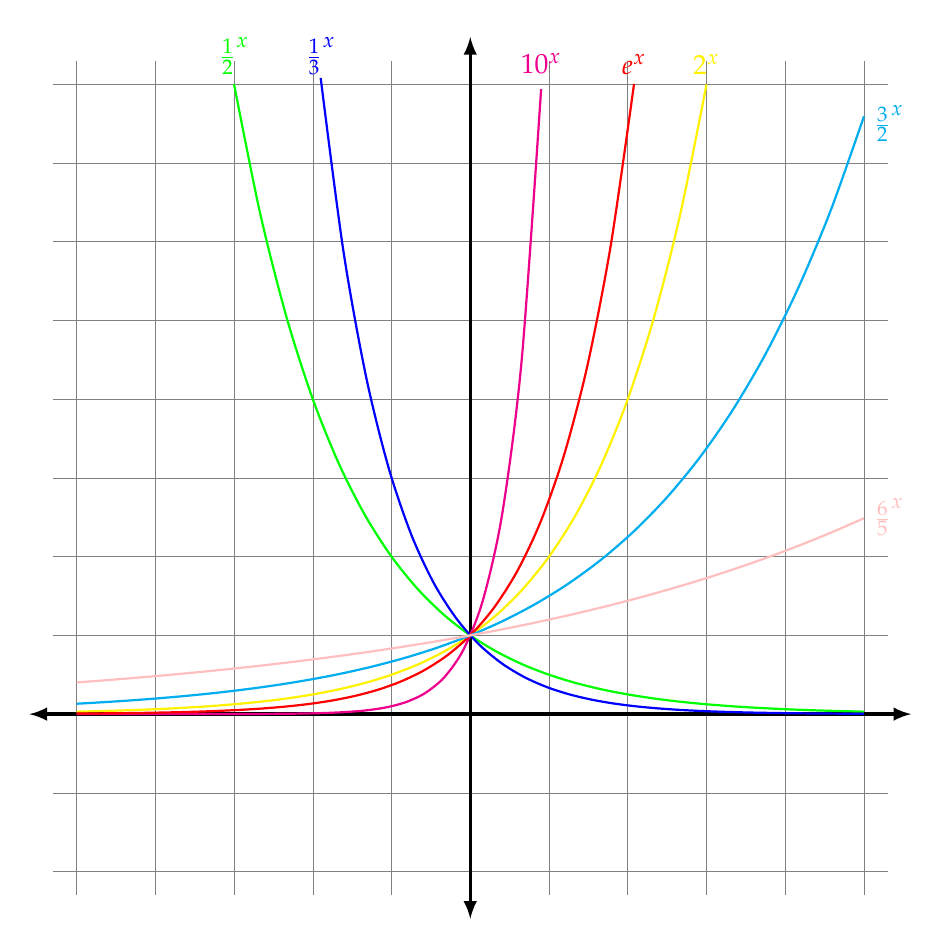
\begin{tikzpicture} 
\draw[gray, very thin] (-5.3,-2.3) grid (5.3,8.3);
\draw[latex-latex, very thick] (-5.6,0)--(5.6,0);
\draw[latex-latex, very thick] (0,-2.6)--(0,8.6);

\draw[domain=-3:5,smooth,variable=\x, green,  thick] plot ({\x},{0.5^\x});
\node[above,green] at (-3,8) {$\frac{1}{2}^x$};

\draw[domain=-1.9:5,smooth,variable=\x, blue,  thick] plot ({\x},{0.333^\x});
\node[above,blue] at (-1.9,8) {$\frac{1}{3}^x$};

\draw[domain=-5:0.9,smooth,variable=\x, magenta,  thick] plot ({\x},{10^\x});
\node[above,magenta] at (0.9,8) {$10^x$}; 

\draw[domain=-5:3,smooth,variable=\x, yellow,  thick] plot ({\x},{2^\x});
\node[above,yellow] at (3,8) {$2^x$};

\draw[domain=-5:2.08,smooth,variable=\x, red,  thick] plot ({\x},{exp(\x)});
\node[above,red] at (2.08,8) {$e^x$};

\draw[domain=-5:5,smooth,variable=\x, cyan,  thick] plot ({\x},{1.5^\x});
\node[right,cyan] at (5,7.5) {$\frac{3}{2}^x$};

\draw[domain=-5:5,smooth,variable=\x, pink,  thick] plot ({\x},{1.2^\x});
\node[right,pink] at (5,2.5) {$\frac{6}{5}^x$};
\end{tikzpicture} 
}

    \item\adjustbox{valign=t}{ 
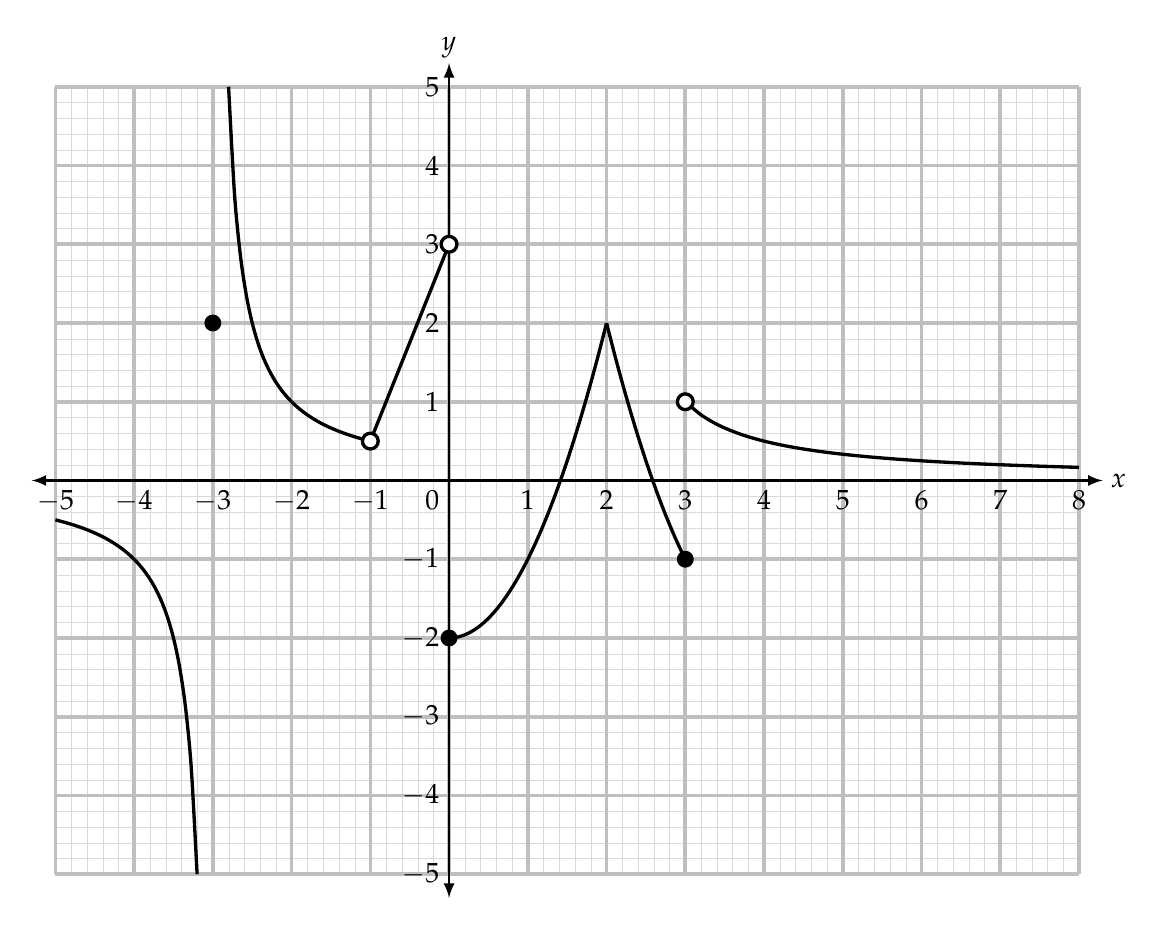
\begin{tikzpicture} 
    \def \minx {-5}
    \def \maxx {8}
    \def \miny {-5}
    \def \maxy {5}


    \draw[black!15, line width=0.05pt,  step=0.2] (\minx,\miny) grid (\maxx,\maxy);
    \draw[black!25, line width=1.3pt, step=1] (\minx,\miny) grid (\maxx,\maxy);


    \draw[thick, latex-latex] (\minx-0.3,0)--(\maxx+0.3,0);
    \draw[thick, latex-latex] (0,\miny-0.3)--(0,\maxy+0.3);
    \node at (\maxx+0.5,0) {$x$};
    \node at (0,\maxy+0.5) {$y$};

    \foreach \x in {\minx,...,-1}
     \node[below,black] at (\x,0) {$\x$};
    \foreach \x in {1,2,...,\maxx}
     \node[below,black] at (\x,0) {$\x$};
    \foreach \y in {\miny,...,-1}
     \node[left,black] at (0,\y) {$\y$};
    \foreach \y in {1,2,...,\maxy}
     \node[left,black] at (0,\y) {$\y$};
    \node[below left,black] at (0,0) {$0$};

    \draw[very thick, domain=-5:-3.2, smooth,variable=\x]  plot ({\x},{1/(\x+3)});
    \draw[very thick, domain=-2.8:-1, smooth,variable=\x]  plot ({\x},{1/(\x+3)});
    \draw[very thick, domain=-1:0, smooth,variable=\x]  plot ({\x},{2.5*\x+3});
    \draw[very thick, domain=0:2, smooth,variable=\x]  plot ({\x},{\x*\x - 2});
    \draw[very thick, domain=2:3, smooth,variable=\x]  plot ({\x},{(\x-4)*(\x-4) - 2});
    \draw[very thick, domain=3:8, smooth,variable=\x]  plot ({\x},{1/(\x-2)});

    \draw [very thick,fill=white] (0,3) circle [radius=0.1];
    \draw [very thick,fill=white] (3,1) circle [radius=0.1];
    \draw [very thick,fill=white] (-1,.5) circle [radius=0.1];
    \draw [fill] (0,-2) circle [radius=0.1];
    \draw [fill] (3,-1) circle [radius=0.1];
  	\draw [fill] (-3,2) circle [radius=0.1];
\end{tikzpicture}
}

\item\adjustbox{valign=t}{
\begin{tikzpicture}[line cap=round, line join=round, >=triangle 45,
                            x=4.0cm, y=1.0cm, scale=1]
          \draw [->,color=black] (-0.1,0) -- (2.5,0);
          \foreach \x in {1,2}
            \draw [shift={(\x,0)}, color=black] (0pt,2pt)
                  -- (0pt,-2pt) node [below] {\footnotesize $\x$};
          \draw [color=black] (2.5,0) node [below] {$x$};
          \draw [->,color=black] (0,-0.1) -- (0,4.5);
          \foreach \y in {1,2,3,4}
            \draw [shift={(0,\y)}, color=black] (2pt,0pt)
                  -- (-2pt,0pt) node[left] {\footnotesize $\y$};
          \draw [color=black] (0,4.5) node [right] {$y$};
          \draw [color=black] (0pt,-10pt) node [left] {\footnotesize $0$};
          \draw [domain=0:2.2, line width=1.0pt] plot (\x,{(\x)^2});
          \clip(0,-0.5) rectangle (3,5);
          \draw (2,0) -- (2,4);
          \foreach \i in {1,...,\thehigher}
            \draw [fill=black,fill opacity=0.3, smooth,samples=50] ({1+(\i-1)/\thehigher},{(1+(\i)/\thehigher)^2})
                  --({1+(\i)/\thehigher},{(1+(\i)/\thehigher)^2})
                  --  ({1+(\i)/\thehigher},0)
                  -- ({1+(\i-1)/\thehigher},0)
                  -- cycle;
        \end{tikzpicture}
}

\item \adjustbox{valign=t}{
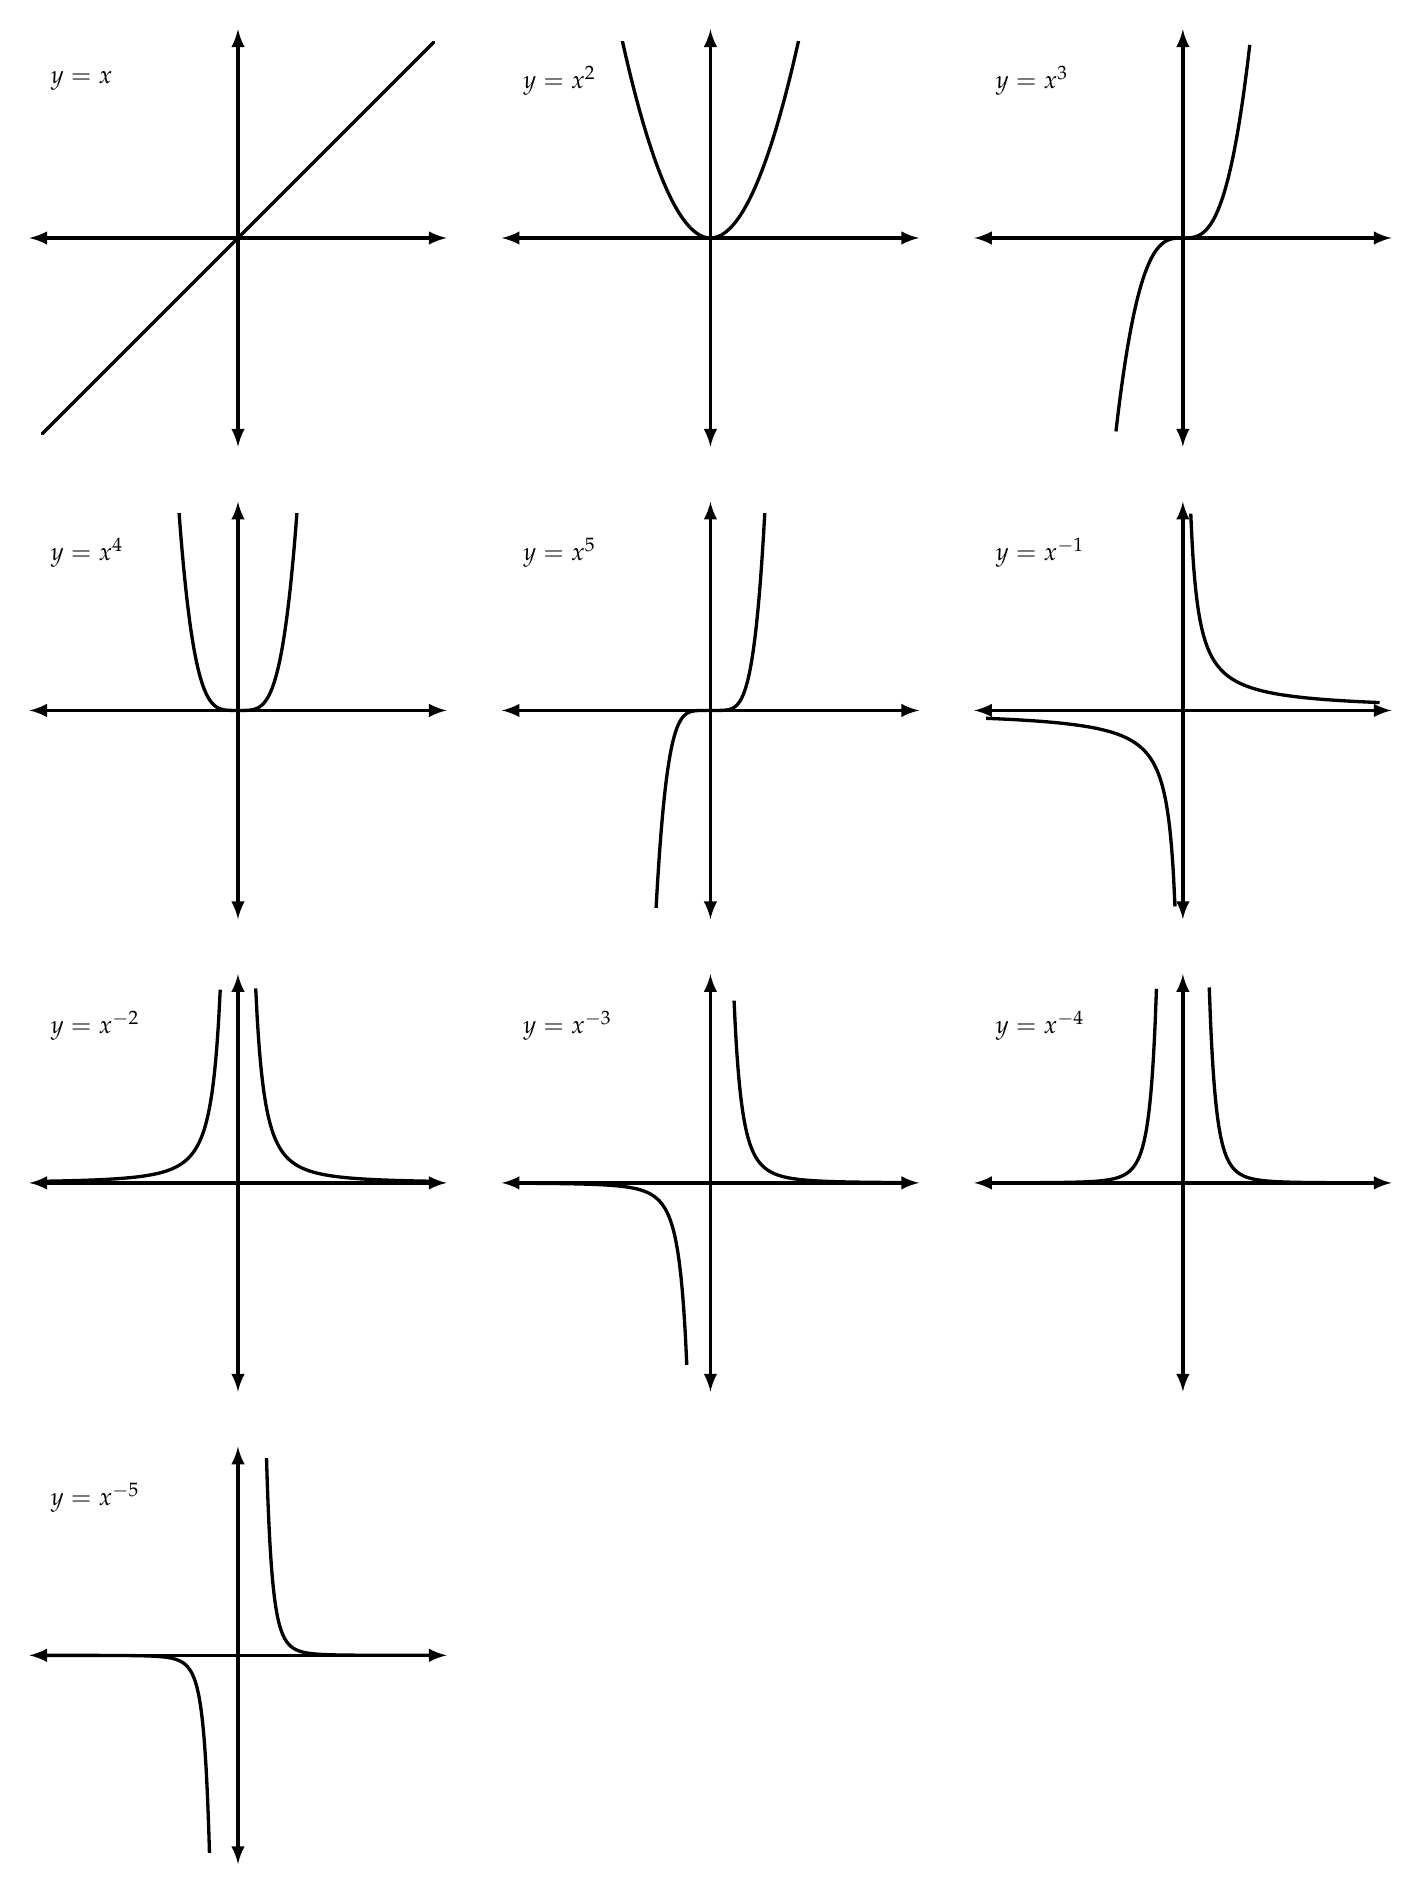
\begin{tikzpicture} 
\foreach \e/\d [count=\i] in {1/5,2/2.3,3/1.7,4/1.5,5/1.5,-1/0.2,-2/0.45,-3/0.6,-4/0.67,-5/0.7} {

  % Compute row and column for 3 graphs per row
  \pgfmathtruncatemacro\col{mod(\i-1, 3)}
  \pgfmathtruncatemacro\row{int((\i-1)/3)}

  \begin{scope}[scale=0.5, xshift=\col*12cm, yshift=-\row*12cm] 
    \ifnum\e = 1
      \node[right] at (-5,4) {\small $y = x$};
    \else 
      \node[right] at (-5,4) {\small $y = x^{\e}$};
    \fi

    \draw[latex-latex, very thick] (-5.3,0)--(5.3,0);
    \draw[latex-latex, very thick] (0,-5.3)--(0,5.3);

    \begin{scope}
      \clip(-5,-5) rectangle (5,5);
      \ifnum\e > 0
        \draw[domain=-\d:\d, smooth, variable=\x, black, samples=120, very thick] plot ({\x},{(\x)^(\e)});
      \else 
        \draw[domain=-5:-\d, smooth, variable=\x, black, samples=120, very thick] plot ({\x},{(\x)^(\e)});
        \draw[domain=\d:5, smooth, variable=\x, black, samples=120, very thick] plot ({\x},{(\x)^(\e)});
      \fi 
    \end{scope}
  \end{scope}
}
\end{tikzpicture}
}












































\item\adjustbox{valign=t}{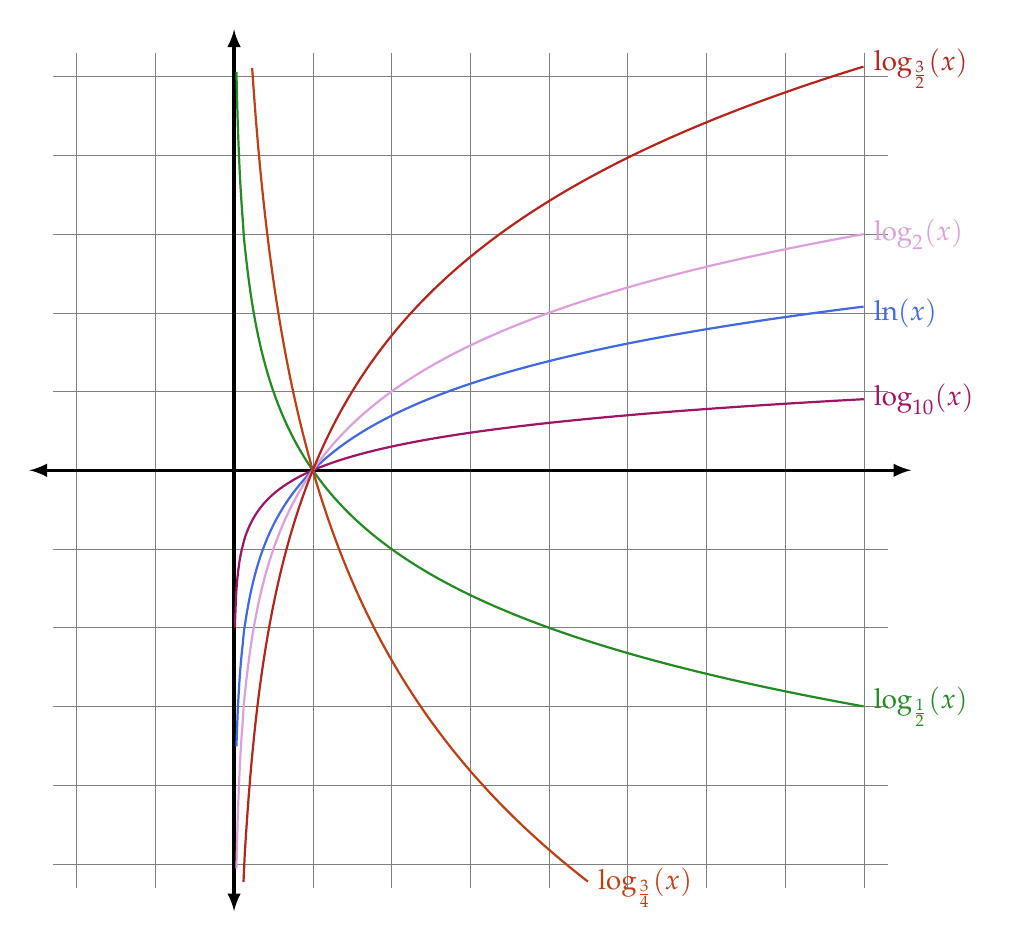
\begin{tikzpicture} 
\draw[Gray, very thin] (-2.3,-5.3) grid (8.3,5.3);
\draw[latex-latex, very thick] (-2.6,0)--(8.6,0);
\draw[latex-latex, very thick] (0,-5.6)--(0,5.6);

 
\draw[domain=0.03:8,smooth,samples=500,variable=\x, ForestGreen,  thick,yscale=-1] plot ({\x},{log2(\x)});
\node[right,ForestGreen] at (8,-3) {$\log_{\frac{1}{2}}(x)$};

\draw[domain=0.23:4.5,smooth,samples=500,variable=\x, Bittersweet,  thick ] plot ({\x},{ln(\x)/ln(0.75)});
\node[right,Bittersweet] at (4.5,-5.3) {$\log_{\frac{3}{4}}(x)$};

\draw[domain=0.01:8,smooth,samples=500,variable=\x, RedViolet,  thick] plot ({\x},{log10(\x)});
\node[right,RedViolet] at (8,0.9) {$\log_{10}(x)$};

\draw[domain=0.03:8,smooth,samples=500,variable=\x, RoyalBlue,  thick] plot ({\x},{ln(\x)});
\node[right,RoyalBlue] at (8,2) {$\ln(x)$};

\draw[domain=0.03:8,smooth,samples=500,variable=\x, Plum,  thick] plot ({\x},{log2(\x)});
\node[right,Plum] at (8,3) {$\log_{2}(x)$};
 
\draw[domain=0.12:8,smooth,samples=500,variable=\x, BrickRed,  thick] plot ({\x},{ln(\x)/ln(1.5)});
\node[right,BrickRed] at (8,5.1) {$\log_{\frac{3}{2}}(x)$};
\end{tikzpicture} }


\item\adjustbox{valign=t}{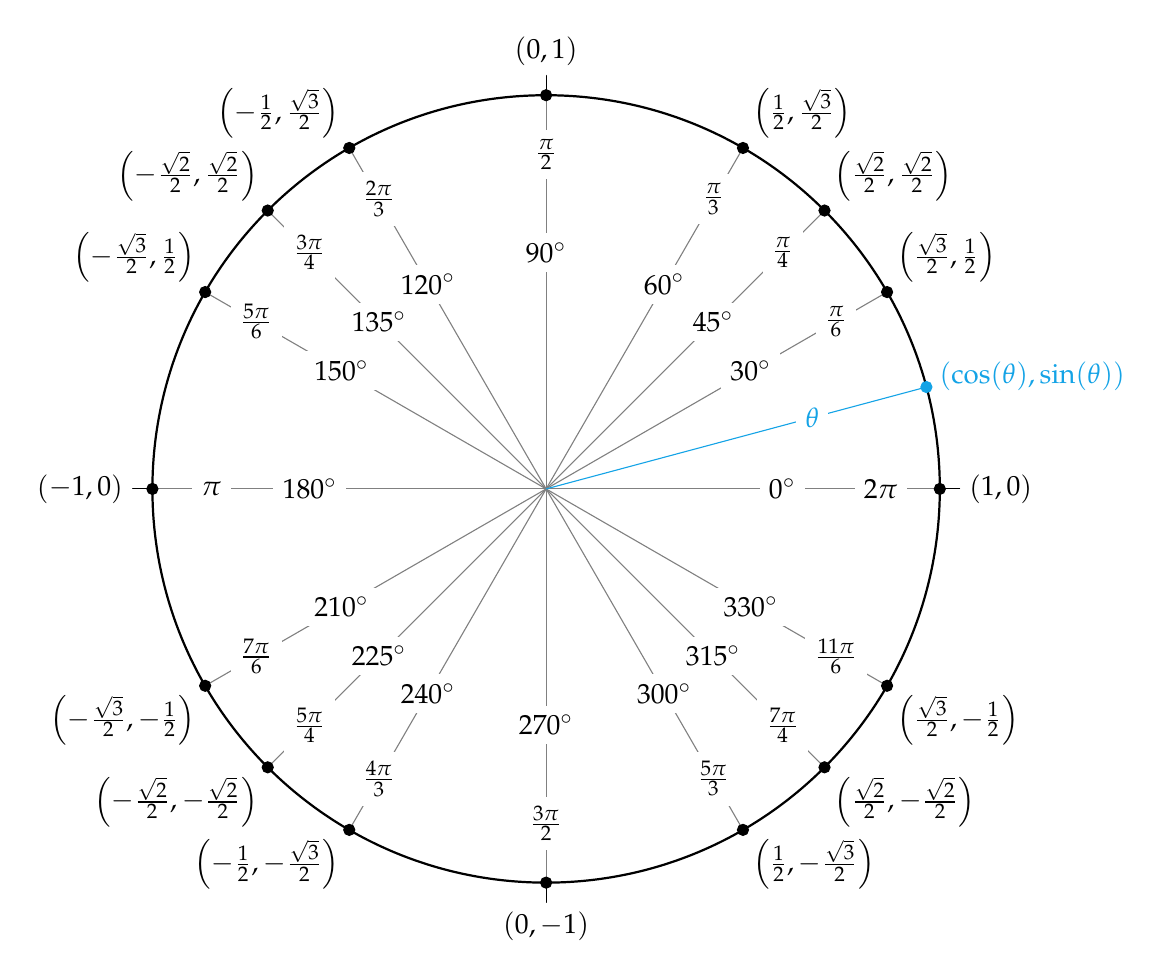
\begin{tikzpicture}[scale=5,cap=round,>=latex]
        % draw the coordinates
        \draw[-] (-1.05cm,0cm) -- (1.05cm,0cm);
        \draw[-] (0cm,-1.05cm) -- (0cm,1.05cm);

        % draw the unit circle
        \draw[thick] (0cm,0cm) circle(1cm);

        \foreach \x in {0,30,45,60,90,120,135,150,180,210,225,240,270,300,315,330} {
                % lines from center to point
                \draw[gray] (0cm,0cm) -- (\x:1cm);
                % dots at each point
                \filldraw[black] (\x:1cm) circle(0.4pt);
                % draw each angle in degrees
                \draw (\x:0.6cm) node[fill=white] {$\x^\circ$};
        }

        \draw[Cerulean](0cm,0cm) -- (15:1cm);
        \filldraw[Cerulean] (15:1cm) circle(0.4pt);
        \draw (15:0.7cm) node[Cerulean,fill=white] {$\theta$};
        \draw (13:1cm) node[above right,Cerulean] {$\left(\cos(\theta), \sin(\theta)\right)$};

        % draw each angle in radians
        \foreach \x/\xtext in {
            30/\frac{\pi}{6},
            45/\frac{\pi}{4},
            60/\frac{\pi}{3},
            90/\frac{\pi}{2},
            120/\frac{2\pi}{3},
            135/\frac{3\pi}{4},
            150/\frac{5\pi}{6},
            180/\pi,
            210/\frac{7\pi}{6},
            225/\frac{5\pi}{4},
            240/\frac{4\pi}{3},
            270/\frac{3\pi}{2},
            300/\frac{5\pi}{3},
            315/\frac{7\pi}{4},
            330/\frac{11\pi}{6},
            360/2\pi}
                \draw (\x:0.85cm) node[fill=white] {$\xtext$};

        \node[right] at (0:1.05cm) {$\left(1,0\right)$};
        \node[above] at (90:1.05cm) {$\left(0,1\right)$};
        \node[left] at (180:1.05cm) {$\left(-1,0\right)$};
        \node[below] at (270:1.05cm) {$\left(0,-1\right)$};

        \foreach \x/\xtext/\y in {
            150/-\frac{\sqrt{3}}{2}/\frac{1}{2},
            135/-\frac{\sqrt{2}}{2}/\frac{\sqrt{2}}{2},
            120/-\frac{1}{2}/\frac{\sqrt{3}}{2}}
                \draw (\x:1cm) node[above left] {$\left(\xtext,\y\right)$};

        
        \foreach \x/\xtext/\y in {
            30/\frac{\sqrt{3}}{2}/\frac{1}{2},
            45/\frac{\sqrt{2}}{2}/\frac{\sqrt{2}}{2},
            60/\frac{1}{2}/\frac{\sqrt{3}}{2}}
                \draw (\x:1cm) node[above right] {$\left(\xtext,\y\right)$}; 
        
        \foreach \x/\xtext/\y in { 
            210/-\frac{\sqrt{3}}{2}/-\frac{1}{2},
            225/-\frac{\sqrt{2}}{2}/-\frac{\sqrt{2}}{2},
            240/-\frac{1}{2}/-\frac{\sqrt{3}}{2} }
                \draw (\x:1cm) node[below left] {$\left(\xtext,\y\right)$};

        \foreach \x/\xtext/\y in {
            330/\frac{\sqrt{3}}{2}/-\frac{1}{2},
            315/\frac{\sqrt{2}}{2}/-\frac{\sqrt{2}}{2},
            300/\frac{1}{2}/-\frac{\sqrt{3}}{2}}
                \draw (\x:1cm) node[below right] {$\left(\xtext,\y\right)$};
 
    \end{tikzpicture}
}


\item\adjustbox{valign=t}{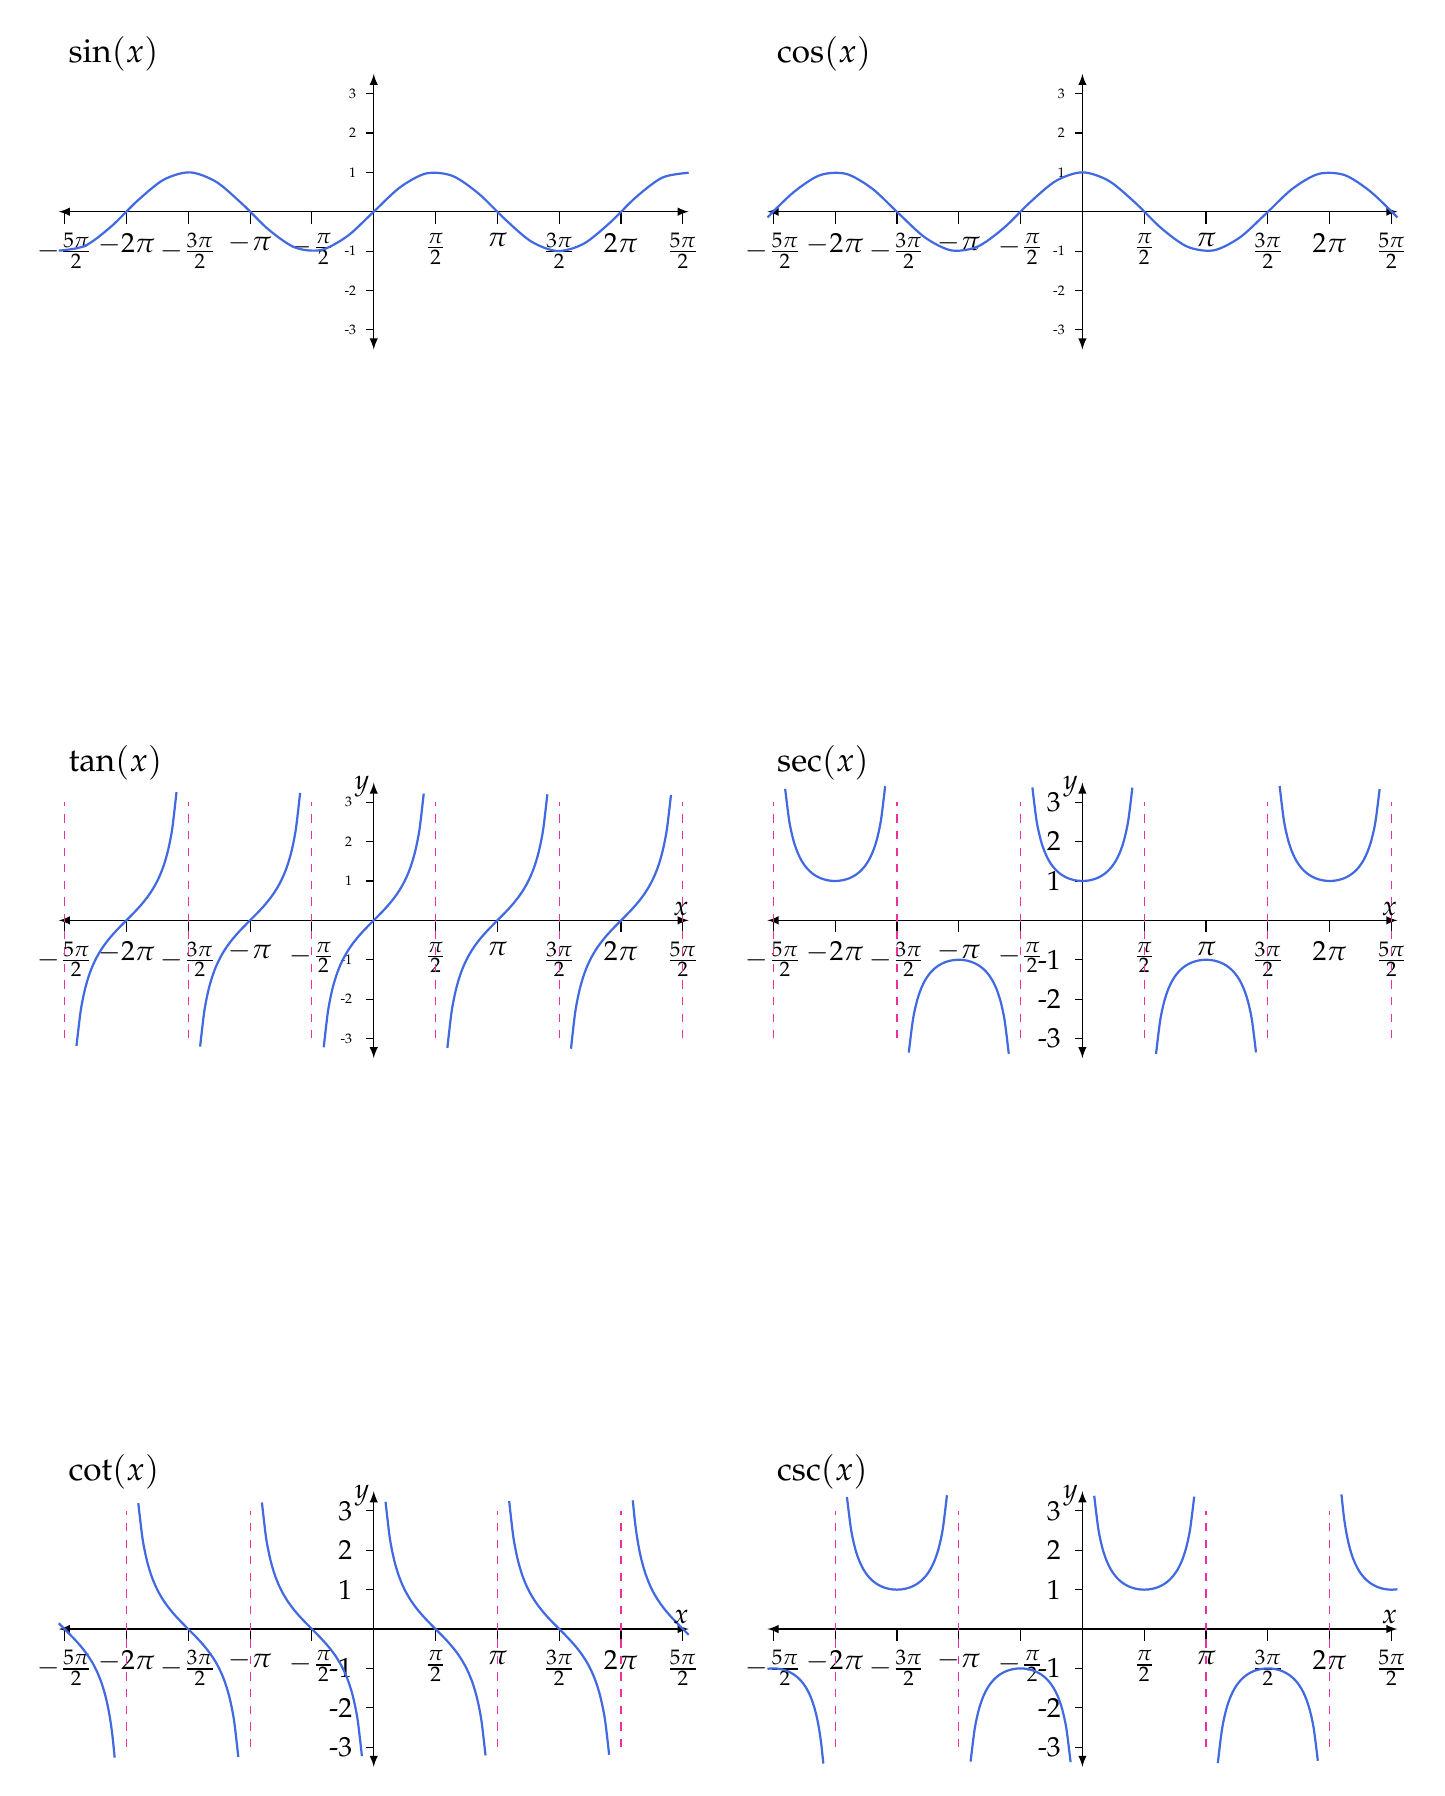
\begin{tikzpicture}[scale=0.5]
%sin
\begin{scope}
\draw[black,latex-latex] (-8,0)--(8,0);
\draw[black,latex-latex] (0,-3.5)--(0,3.5);

\foreach \x/\l in {-7.85/$-\frac{5\pi}{2}$,-6.28/$-2\pi$,-4.71/$-\frac{3\pi}{2}$,-3.14/$-\pi$,-1.57/$-\frac{\pi}{2}$,1.57/$\frac{\pi}{2}$,3.14/$\pi$,4.71/$\frac{3\pi}{2}$, 6.28/$2\pi$,7.85/$\frac{5\pi}{2}$} {
  \node[below] at (\x,-0.3) {\l};
  \draw[black] (\x,0)--(\x,-0.3);
}
\foreach \y in {-3,-2,-1,1,2,3} {
  \node[left] at (-0.2,\y) {\tiny \y};
  \draw[black] (-0.2,\y)--(0,\y);
}

\draw[ thick,RoyalBlue,domain=-8:8,smooth] plot (\x,{sin(deg(\x))});
\node[right] at (-8,4) {\large $\sin(x)$};
\end{scope}
 
 % tan
\begin{scope}[yshift=-18cm]
    \draw[black,latex-latex] (-8,0)--(8,0);
    \draw[black,latex-latex] (0,-3.5)--(0,3.5);

    \foreach \x/\l in {-7.85/$-\frac{5\pi}{2}$,-6.28/$-2\pi$,-4.71/$-\frac{3\pi}{2}$,-3.14/$-\pi$,-1.57/$-\frac{\pi}{2}$,1.57/$\frac{\pi}{2}$,3.14/$\pi$,4.71/$\frac{3\pi}{2}$, 6.28/$2\pi$,7.85/$\frac{5\pi}{2}$} {
      \node[below] at (\x,-0.3) {\l};
      \draw[black] (\x,0)--(\x,-0.3);
    }
    \foreach \y in {-3,-2,-1,1,2,3} {
      \node[left] at (-0.3,\y) {\tiny \y};
      \draw[black] (-0.2,\y)--(0,\y);
    }

    \draw[  thick,RoyalBlue,domain=-7.55:-5.01,smooth] plot (\x,{tan(deg(\x))});
    \draw[  thick,RoyalBlue,domain=-4.41:-1.87,smooth] plot (\x,{tan(deg(\x))});
    \draw[  thick,RoyalBlue,domain=-1.27:1.27,smooth] plot (\x,{tan(deg(\x))});
    \draw[  thick,RoyalBlue,domain=1.87:4.41,smooth] plot (\x,{tan(deg(\x))});
    \draw[  thick,RoyalBlue,domain=5.01:7.55,smooth] plot (\x,{tan(deg(\x))});

    \draw[Rhodamine,dashed] (1.57,-3)--(1.57,3);
    \draw[Rhodamine,dashed] (4.71,-3)--(4.71,3);
    \draw[Rhodamine,dashed] (7.85,-3)--(7.85,3);
    \draw[Rhodamine,dashed] (-1.57,-3)--(-1.57,3);
    \draw[Rhodamine,dashed] (-4.71,-3)--(-4.71,3);
    \draw[Rhodamine,dashed] (-7.85,-3)--(-7.85,3);


    \node at (7.8,0.3) {$x$};
    \node at (-0.3,3.4) {$y$};
    \node[right] at (-8,4) {\large $\tan(x)$};
\end{scope}
 
 % sec
\begin{scope}[xshift=18cm,yshift=-18cm]
    \draw[black,latex-latex] (-8,0)--(8,0);
    \draw[black,latex-latex] (0,-3.5)--(0,3.5);

    \foreach \x/\l in {-7.85/$-\frac{5\pi}{2}$,-6.28/$-2\pi$,-4.71/$-\frac{3\pi}{2}$,-3.14/$-\pi$,-1.57/$-\frac{\pi}{2}$,1.57/$\frac{\pi}{2}$,3.14/$\pi$,4.71/$\frac{3\pi}{2}$, 6.28/$2\pi$,7.85/$\frac{5\pi}{2}$} {
      \node[below] at (\x,-0.3) {\l};
      \draw[black] (\x,0)--(\x,-0.3);
    }
    \foreach \y in {-3,-2,-1,1,2,3} {
      \node[left] at (-0.3,\y) {\y};
      \draw[black] (-0.2,\y)--(0,\y);
    }

    \draw[  thick,RoyalBlue,domain=-7.55:-5.01,smooth] plot (\x,{sec(deg(\x))});
    \draw[  thick,RoyalBlue,domain=-4.41:-1.87,smooth] plot (\x,{sec(deg(\x))});
    \draw[  thick,RoyalBlue,domain=-1.27:1.27,smooth] plot (\x,{sec(deg(\x))});
    \draw[  thick,RoyalBlue,domain=1.87:4.41,smooth] plot (\x,{sec(deg(\x))});
    \draw[  thick,RoyalBlue,domain=5.01:7.55,smooth] plot (\x,{sec(deg(\x))});

    \draw[Rhodamine,dashed] (1.57,-3)--(1.57,3);
    \draw[Rhodamine,dashed] (4.71,-3)--(4.71,3);
    \draw[Rhodamine,dashed] (7.85,-3)--(7.85,3);
    \draw[Rhodamine,dashed] (-1.57,-3)--(-1.57,3);
    \draw[Rhodamine,dashed] (-4.71,-3)--(-4.71,3);
    \draw[Rhodamine,dashed] (-7.85,-3)--(-7.85,3);

    \node at (7.8,0.3) {$x$};
    \node at (-0.3,3.4) {$y$};
    \node[right] at (-8,4) {\large $\sec(x)$};
\end{scope}
 
 %cos
\begin{scope}[xshift=18cm]
    \draw[black,latex-latex] (-8,0)--(8,0);
    \draw[black,latex-latex] (0,-3.5)--(0,3.5);

    \foreach \x/\l in {-7.85/$-\frac{5\pi}{2}$,-6.28/$-2\pi$,-4.71/$-\frac{3\pi}{2}$,-3.14/$-\pi$,-1.57/$-\frac{\pi}{2}$,1.57/$\frac{\pi}{2}$,3.14/$\pi$,4.71/$\frac{3\pi}{2}$, 6.28/$2\pi$,7.85/$\frac{5\pi}{2}$} {
      \node[below] at (\x,-0.3) {\l};
      \draw[black] (\x,0)--(\x,-0.3);
    }
    \foreach \y in {-3,-2,-1,1,2,3} {
      \node[left] at (-0.2,\y) {\tiny \y};
      \draw[black] (-0.2,\y)--(0,\y);
    }

    \draw[ thick,RoyalBlue,domain=-8:8,smooth] plot (\x,{cos(deg(\x))});
    \node[right] at (-8,4) {\large $\cos(x)$};
\end{scope}
 
 % cot
\begin{scope}[yshift=-36cm] 
    \draw[black,latex-latex] (-8,0)--(8,0);
    \draw[black,latex-latex] (0,-3.5)--(0,3.5);

    \foreach \x/\l in {-7.85/$-\frac{5\pi}{2}$,-6.28/$-2\pi$,-4.71/$-\frac{3\pi}{2}$,-3.14/$-\pi$,-1.57/$-\frac{\pi}{2}$,1.57/$\frac{\pi}{2}$,3.14/$\pi$,4.71/$\frac{3\pi}{2}$, 6.28/$2\pi$,7.85/$\frac{5\pi}{2}$} {
      \node[below] at (\x,-0.3) {\l};
      \draw[black] (\x,0)--(\x,-0.3);
    }
    \foreach \y in {-3,-2,-1,1,2,3} {
      \node[left] at (-0.3,\y) {\y};
      \draw[black] (-0.2,\y)--(0,\y);
    }

    \draw[  thick,RoyalBlue,domain=-8:-6.58,smooth] plot (\x,{cot(deg(\x))});
    \draw[  thick,RoyalBlue,domain=-5.98:-3.44,smooth] plot (\x,{cot(deg(\x))});
    \draw[  thick,RoyalBlue,domain=-2.84:-0.3,smooth] plot (\x,{cot(deg(\x))});
    \draw[  thick,RoyalBlue,domain=0.3:2.84,smooth] plot (\x,{cot(deg(\x))});
    \draw[  thick,RoyalBlue,domain=3.44:5.98,smooth] plot (\x,{cot(deg(\x))});
    \draw[  thick,RoyalBlue,domain=6.58:8,smooth] plot (\x,{cot(deg(\x))});


    \draw[Rhodamine,dashed] (3.14,-3)--(3.14,3);
    \draw[Rhodamine,dashed] (6.28,-3)--(6.28,3);
     \draw[Rhodamine,dashed] (-3.14,-3)--(-3.14,3);
    \draw[Rhodamine,dashed] (-6.28,-3)--(-6.28,3);


    \node at (7.8,0.3) {$x$};
    \node at (-0.3,3.4) {$y$};
    \node[right] at (-8,4) {\large $\cot(x)$};
\end{scope}
 
 %csc
\begin{scope}[xshift=18cm,yshift=-36cm] 
    \draw[black,latex-latex] (-8,0)--(8,0);
    \draw[black,latex-latex] (0,-3.5)--(0,3.5);

    \foreach \x/\l in {-7.85/$-\frac{5\pi}{2}$,-6.28/$-2\pi$,-4.71/$-\frac{3\pi}{2}$,-3.14/$-\pi$,-1.57/$-\frac{\pi}{2}$,1.57/$\frac{\pi}{2}$,3.14/$\pi$,4.71/$\frac{3\pi}{2}$, 6.28/$2\pi$,7.85/$\frac{5\pi}{2}$} {
      \node[below] at (\x,-0.3) {\l};
      \draw[black] (\x,0)--(\x,-0.3);
    }
    \foreach \y in {-3,-2,-1,1,2,3} {
      \node[left] at (-0.3,\y) {\y};
      \draw[black] (-0.2,\y)--(0,\y);
    }

    \draw[  thick,RoyalBlue,domain=-8:-6.58,smooth] plot (\x,{cosec(deg(\x))});
    \draw[  thick,RoyalBlue,domain=-5.98:-3.44,smooth] plot (\x,{cosec(deg(\x))});
    \draw[  thick,RoyalBlue,domain=-2.84:-0.3,smooth] plot (\x,{cosec(deg(\x))});
    \draw[  thick,RoyalBlue,domain=0.3:2.84,smooth] plot (\x,{cosec(deg(\x))});
    \draw[  thick,RoyalBlue,domain=3.44:5.98,smooth] plot (\x,{cosec(deg(\x))});
    \draw[  thick,RoyalBlue,domain=6.58:8,smooth] plot (\x,{cosec(deg(\x))});


    \draw[Rhodamine,dashed] (3.14,-3)--(3.14,3);
    \draw[Rhodamine,dashed] (6.28,-3)--(6.28,3);
     \draw[Rhodamine,dashed] (-3.14,-3)--(-3.14,3);
    \draw[Rhodamine,dashed] (-6.28,-3)--(-6.28,3);

    \node at (7.8,0.3) {$x$};
    \node at (-0.3,3.4) {$y$};
    \node[right] at (-8,4) {\large $\csc(x)$};
    \end{scope}
  \end{tikzpicture}}


\item\adjustbox{valign=t}{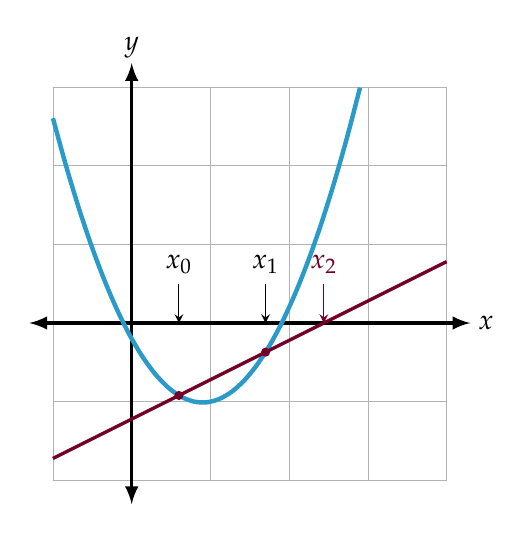
\begin{tikzpicture} 
  \draw[black!30, very thin] (-1,-2) grid (4,3);
  \draw[latex-latex, very thick] (-1.3,0)--(4.3,0);
  \draw[latex-latex, very thick] (0,-2.3)--(0,3.3);
  \node at (4.5,0) {$x$};
  \node at (0,3.5) {$y$};

  \draw[domain=-1:2.9,smooth,variable=\x, cyan!80!black, ultra thick] plot ({\x},{\x*\x -1.8*\x-0.2});

  \node[above] at (0.6,0.5) { $x_0$};
  \node[above] at (1.7,0.5) { $x_1$};
  \draw[-stealth] (0.6,0.5)--(0.6,0);
  \draw[-stealth] (1.7,0.5)--(1.7,0);

  \node[above, purple!60!black] at (2.44,0.5) { $x_2$};
  \draw[-stealth, purple!60!black] (2.44,0.5)--(2.44,0);

  \draw [fill, purple!60!black] (0.6,-0.92) circle [radius=0.05];
  \draw [fill, purple!60!black] (1.7,-0.37) circle [radius=0.05];
  \draw[purple!60!black, very thick] (-1,-1.72)--(4,0.78);
\end{tikzpicture}}

\item\adjustbox{valign=t}{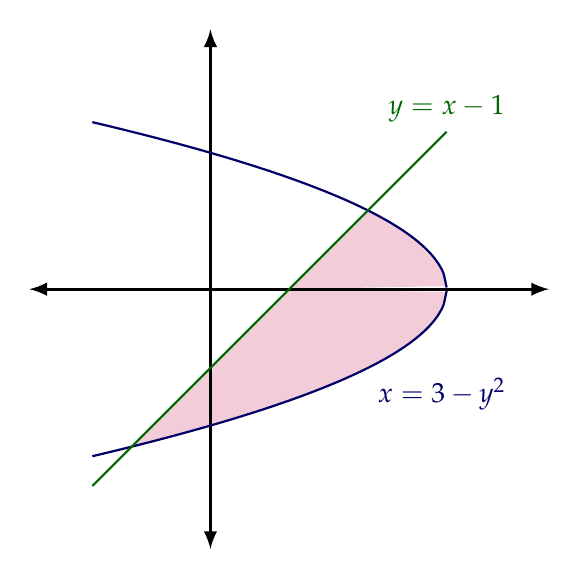
\begin{tikzpicture}
%shading
\fill[domain=2:3,smooth,samples=100,variable=\x, purple!20] plot ({\x},{sqrt(3-\x)})--(1,0);
\fill[domain=-1:3,smooth,samples=100,variable=\x, purple!20] plot ({\x},{-sqrt(3-\x)})--(1,0);

%axes
\draw[latex-latex,very thick] (-2.3,0)--(4.3,0);
\draw[latex-latex,very thick] (0,-3.3)--(0,3.3);

%graphs
\draw[domain=-1.5:3,smooth,samples=120,variable=\x, blue!40!black, thick] plot ({\x},{sqrt(3-\x)});
\draw[domain=-1.5:3,smooth,samples=120,variable=\x, blue!40!black,thick] plot ({\x},{-sqrt(3-\x)});
\draw[domain=-1.5:3,smooth,variable=\x, black, thick, green!40!black] plot ({\x},{\x-1});

%labels
\node [below right,blue!40!black] at (2,-1) {$x=3-y^2$};
\node [above,green!40!black] at (3,2) {$y=x-1$};
\end{tikzpicture}}

\item\adjustbox{valign=t}{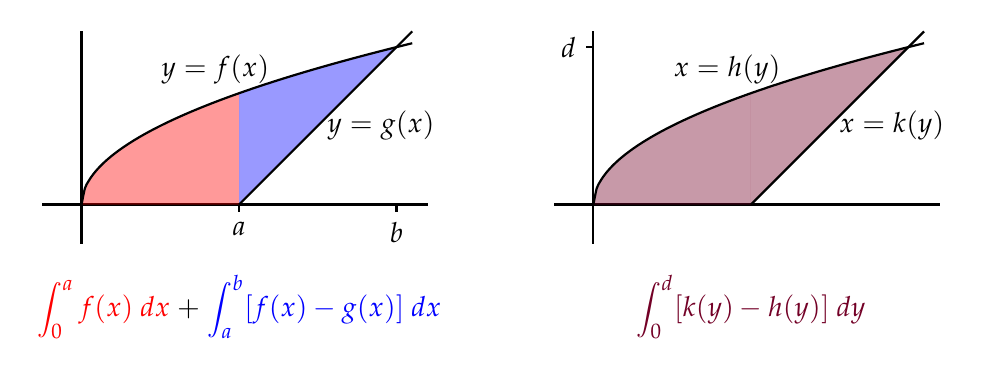
\begin{tikzpicture} 
  \draw[thick ](-0.5,0)--(4.4,0);
  \draw[thick ](0,-0.5)--(0,2.2);
  \draw[thick ](2,0)--(2,-0.1);
  \draw[thick](4,0)--(4,-0.1);
  \node[below] at (2,-0.1) {$a$};
  \node[below] at (4,-0.1) {$b$};

  \fill[ domain=0:2,smooth,variable=\x,red, fill opacity=0.4]  plot ({(\x},{sqrt(\x)})--(2,0);
  \fill[ domain=2:4,smooth,variable=\x,blue, fill opacity=0.4]  plot ({(\x},{sqrt(\x)})--(2,0);

  \draw[thick,domain=0:4.2,smooth,samples=100]  plot ({(\x},{sqrt(\x)});
  \draw[thick,domain=2:4.2,smooth ]  plot ({(\x},{\x-2});
  \node[above,black] at (1.7,1.4) {$y=f(x)$};
  \node[right,black] at (3,1) {$y=g(x)$};
  \node at (2,-1.3) {$\displaystyle \color{red}{\int_0^a f(x) \ dx} \ \color{black}{+} \ \color{blue}{\int_a^b [f(x)-g(x)] \ dx} $}; 
\begin{scope}[xshift=6.5cm]
    \draw[thick](-0.5,0)--(4.4,0);
    \draw[thick](0,-0.5)--(0,2.2);
    \draw[thick](0,2)--(-0.1,2);
    \node[left] at (-0.1,2) {$d$};

    \fill[ domain=0:2,smooth,variable=\x,purple!60!black, fill opacity=0.4]  plot ({(\x},{sqrt(\x)})--(2,0);
    \fill[ domain=2:4,smooth,variable=\x,purple!60!black, fill opacity=0.4]  plot ({(\x},{sqrt(\x)})--(2,0);

    \draw[thick,domain=0:4.2,smooth,samples=100]  plot ({(\x},{sqrt(\x)});
    \draw[thick,domain=2:4.2,smooth ]  plot ({(\x},{\x-2});
    \node[above,black] at (1.7,1.4) {$x=h(y)$};
    \node[right,black] at (3,1) {$x=k(y)$};
    \node at (2,-1.3) {$\displaystyle  \color{purple!60!black}{\int_0^d [k(y)-h(y)] \ dy} $}; 
\end{scope}
\end{tikzpicture}}

\item\adjustbox{valign=t}{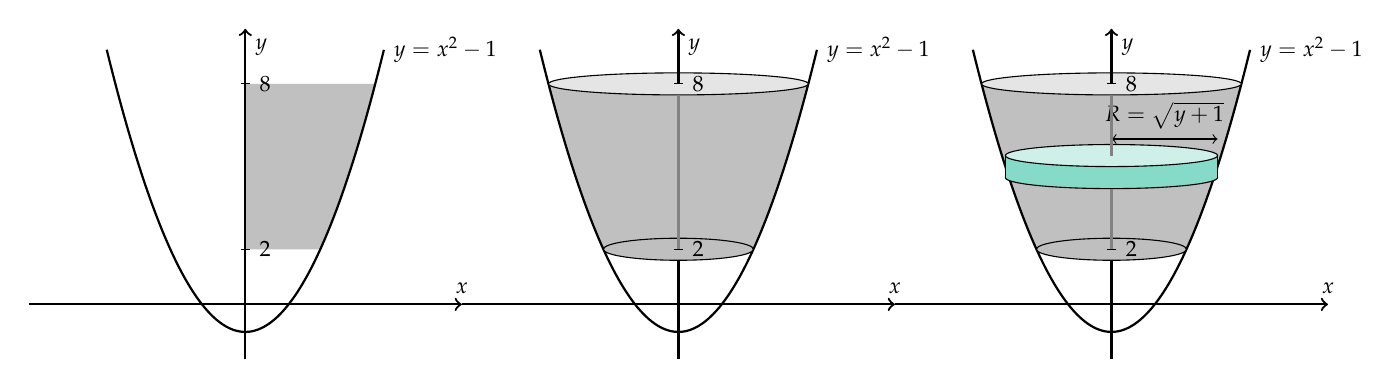
\begin{tikzpicture}[xscale=0.55,yscale=0.7]
    \begin{scope}
      \fill[fill=medgrey, opacity=0.5] (0,1) -- plot[domain=-0:3](\x,{0.5*(\x*\x-1)}) -- (0,4);
      \fill[fill=white] (-1.732050808,1) -- plot[domain=-1.732050808:1.732050808] (\x,{0.5*(\x*\x-1)}) -- (1.732050808,1);

      \draw[-,thick, domain=-3.2:3.2, samples=100] plot (\x,{0.5*(\x*\x-1)}) node[right] {\footnotesize $y=x^2-1$};

      \draw[->, thick] (-5,0) -- (5,0) node[above] {\footnotesize $x$};
      \draw[->, thick] (0,-1) -- (0,5) node[below right]{\footnotesize $y$};
      \draw[-] (-3pt,1) -- (3pt,1) node[right] {\footnotesize $2$};
      \draw[-] (-3pt,4) -- (3pt,4) node[right] {\footnotesize $8$};
    \end{scope}
    \begin{scope}[xshift=10cm]
    \fill[fill=medgrey, opacity=0.5] (-3,4) -- plot[domain=-3:3](\x,{0.5*(\x*\x-1)}) -- (3,4);
    \fill[fill=white] (-1.732050808,1) -- plot[domain=-1.732050808:1.732050808] (\x,{0.5*(\x*\x-1)}) -- (1.732050808,1);

    \draw[-,thick, domain=-3.2:3.2, samples=100] plot (\x,{0.5*(\x*\x-1)}) node[right] {\footnotesize $y=x^2-1$};
    \draw[fill=gray!20] (0,4) circle [y radius =.2 , x radius =3];
    \draw[fill=gray!50] (0,1) circle [y radius =.2 , x radius =1.732050808];


    \draw[->, thick] (-5,0) -- (5,0) node[above] {\footnotesize $x$};
    \draw[thick] (0,-1) -- (0,0.8);
    \draw[thick,medgrey] (0,1) -- (0,3.8);
    \draw[->, thick] (0,4) -- (0,5) node[below right]{\footnotesize $y$};
    \draw[-] (-3pt,1) -- (3pt,1) node[right] {\footnotesize $2$};
    \draw[-] (-3pt,4) -- (3pt,4) node[right] {\footnotesize $8$};
  \end{scope}
    \begin{scope}[xshift=20cm]
    \fill[fill=medgrey, opacity=0.5] (-3,4) -- plot[domain=-3:3](\x,{0.5*(\x*\x-1)}) -- (3,4);
    \fill[fill=white] (-1.732050808,1) -- plot[domain=-1.732050808:1.732050808] (\x,{0.5*(\x*\x-1)}) -- (1.732050808,1);

    \draw[-,thick, domain=-3.2:3.2, samples=100] plot (\x,{0.5*(\x*\x-1)}) node[right] {\footnotesize $y=x^2-1$};
    \draw[fill=gray!20] (0,4) circle [y radius =.2 , x radius =3];
    \draw[fill=gray!50] (0,1) circle [y radius =.2 , x radius =1.732050808];
    \draw[fill=Acolor] (0,2.3) circle [y radius =.2 , x radius =2.449489743];
    \fill[Acolor] (-2.449489743,2.3) rectangle (2.449489743,2.7);
    \draw[fill=Acolor!40] (0,2.7) circle [y radius =.2 , x radius =2.449489743];
    \draw (2.449489743,2.3) -- (2.449489743,2.7);
    \draw (-2.449489743,2.3) -- (-2.449489743,2.7);
    \draw[<->] (0,3) -- (2.449489743,3) node[above, midway]  {\footnotesize $R = \sqrt{y+1}$};
    \draw[->, thick] (-5,0) -- (5,0) node[above] {\footnotesize $x$};
    \draw[thick] (0,-1) -- (0,0.8);
    \draw[thick,medgrey] (0,1) -- (0,2.1);
    \draw[thick,medgrey] (0,2.7) -- (0,3.8);
    \draw[->, thick] (0,4) -- (0,5) node[below right]{\footnotesize $y$};
    \draw[-] (-3pt,1) -- (3pt,1) node[right] {\footnotesize $2$};
    \draw[-] (-3pt,4) -- (3pt,4) node[right] {\footnotesize $8$};
  \end{scope}
    \end{tikzpicture}}


    
\item\adjustbox{valign=t}{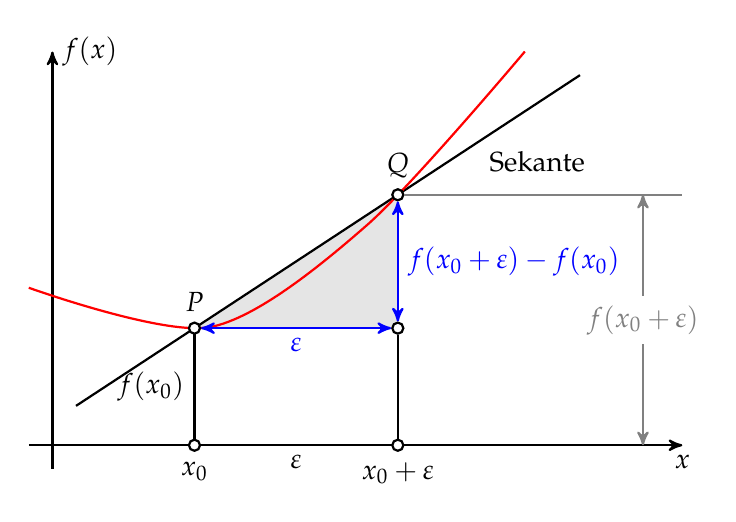
\begin{tikzpicture}[
    thick,
    >=stealth',
    dot/.style = {
      draw,
      fill = white,
      circle,
      inner sep = 0pt,
      minimum size = 4pt
    }
  ]
  \coordinate (O) at (0,0);
  \draw[->] (-0.3,0) -- (8,0) coordinate[label = {below:$x$}] (xmax);
  \draw[->] (0,-0.3) -- (0,5) coordinate[label = {right:$f(x)$}] (ymax);
  \path[name path=x] (0.3,0.5) -- (6.7,4.7);
  \path[name path=y] plot[smooth] coordinates {(-0.3,2) (2,1.5) (4,2.8) (6,5)};
  \scope[name intersections = {of = x and y, name = i}]
    \fill[gray!20] (i-1) -- (i-2 |- i-1) -- (i-2) -- cycle;
    \draw      (0.3,0.5) -- (6.7,4.7) node[pos=0.8, below right] {Sekante};
    \draw[red] plot[smooth] coordinates {(-0.3,2) (2,1.5) (4,2.8) (6,5)};
    \draw (i-1) node[dot, label = {above:$P$}] (i-1) {} -- node[left]
      {$f(x_0)$} (i-1 |- O) node[dot, label = {below:$x_0$}] {};
    \path (i-2) node[dot, label = {above:$Q$}] (i-2) {} -- (i-2 |- i-1)
      node[dot] (i-12) {};
    \draw           (i-12) -- (i-12 |- O) node[dot,
                              label = {below:$x_0 + \varepsilon$}] {};
    \draw[blue, <->] (i-2) -- node[right] {$f(x_0 + \varepsilon) - f(x_0)$}
                              (i-12);
    \draw[blue, <->] (i-1) -- node[below] {$\varepsilon$} (i-12);
    \path       (i-1 |- O) -- node[below] {$\varepsilon$} (i-2 |- O);
    \draw[gray]      (i-2) -- (i-2 -| xmax);
    \draw[gray, <->] ([xshift = -0.5cm]i-2 -| xmax) -- node[fill = white]
      {$f(x_0 + \varepsilon)$}  ([xshift = -0.5cm]xmax);
  \endscope
\end{tikzpicture}}


\end{enumerate}

\section{Graph Theory}

\begin{enumerate}

\item\adjustbox{valign=t}{
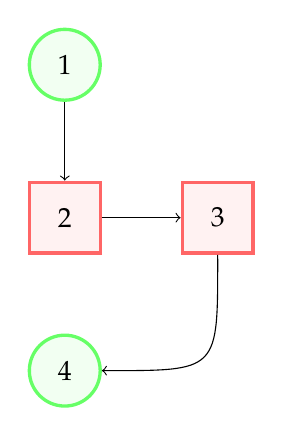
\begin{tikzpicture}[
roundnode/.style={circle, draw=green!60, fill=green!5, very thick, minimum size=9mm},
squarednode/.style={rectangle, draw=red!60, fill=red!5, very thick, minimum size=9mm},
]
%Nodes
\node[squarednode]      (maintopic)                              {2};
\node[roundnode]        (uppercircle)       [above=of maintopic] {1};
\node[squarednode]      (rightsquare)       [right=of maintopic] {3};
\node[roundnode]        (lowercircle)       [below=of maintopic] {4};

%Lines
\draw[->] (uppercircle.south) -- (maintopic.north);
\draw[->] (maintopic.east) -- (rightsquare.west);
\draw[->] (rightsquare.south) .. controls +(down:15mm) and +(right:15mm) .. (lowercircle.east);
\end{tikzpicture}
}



    \item\adjustbox{valign=t}{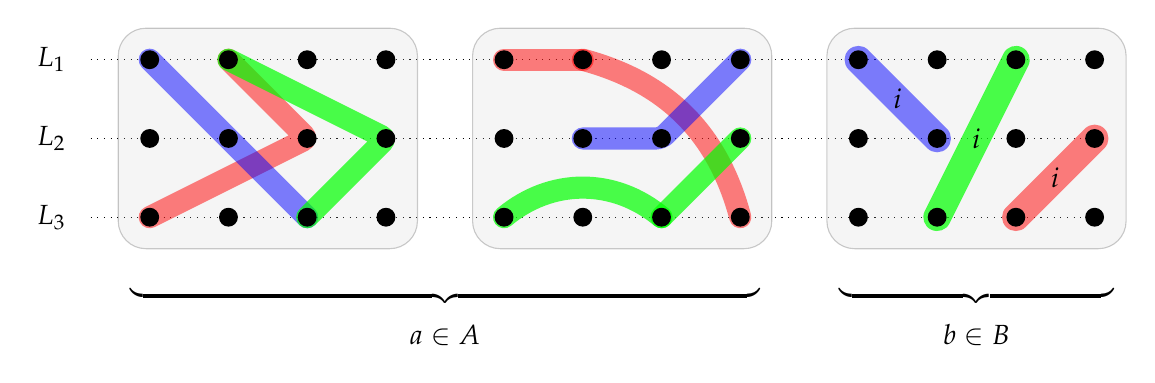
\begin{tikzpicture}

\draw[thin, dotted] (.25,3) to (13,3);
\draw[thin, dotted] (.25,2) to (13,2);
\draw[thin, dotted] (.25,1) to (13,1);

\node at (-.25,3) {$L_1$};
\node at (-.25,2) {$L_2$};
\node at (-.25,1) {$L_3$};

\node at (4.75,0) {$\underbrace{\hspace{8cm}}$};
\node at (4.75,-.5) {$a\in A$};



\begin{scope}[shift = {(0,0)}]
\draw[rounded corners = 10pt, fill = gray!40!, opacity =.2] (1-.4,3+.4) -- (4+.4,3+.4) -- (4+.4,1-.4) -- (1-.4,1-.4) -- cycle;




\draw[rounded corners = 2pt, line width = 8pt, red, line cap = round, opacity = .5] (2,3) -- (3,2) -- (1,1);

\draw[rounded corners = 2pt, line width = 8pt, blue, line cap = round, opacity = .5] (1,3) -- (2,2) -- (3,1);

\draw[rounded corners = 2pt, line width = 8pt, green, line cap = round, opacity = .7] (2,3) -- (4,2) -- (3,1);



\draw[thick, fill = black] (1,3) circle (3pt); 
\draw[thick, fill = black] (2,3) circle (3pt); 
\draw[thick, fill = black] (3,3) circle (3pt); 
\draw[thick, fill = black] (4,3) circle (3pt); 

\draw[thick, fill = black] (1,2) circle (3pt); 
\draw[thick, fill = black] (2,2) circle (3pt); 
\draw[thick, fill = black] (3,2) circle (3pt); 
\draw[thick, fill = black] (4,2) circle (3pt); 

\draw[thick, fill = black] (1,1) circle (3pt); 
\draw[thick, fill = black] (2,1) circle (3pt); 
\draw[thick, fill = black] (3,1) circle (3pt); 
\draw[thick, fill = black] (4,1) circle (3pt); 


\end{scope}

%%%%%%%%%%%%%%%%%%%%%%%%%%%%%%%%

\begin{scope}[shift = {(4.5,0)}]


\draw[rounded corners = 10pt, fill = gray!40!, opacity =.2] (1-.4,3+.4) -- (4+.4,3+.4) -- (4+.4,1-.4) -- (1-.4,1-.4) -- cycle;


\draw[rounded corners = 2pt, line width = 8pt, red, line cap = round, opacity =.5] (1,3) -- (2,3);
\draw[rounded corners = 2pt, line width = 8pt, red, line cap = round, bend left = 30, opacity = .5] (2,3) to (4,1);

\draw[rounded corners = 2pt, line width = 8pt, blue, line cap = round, bend left = 30, opacity = .5] (4,3) -- (3,2) -- (2,2);

\draw[rounded corners = 2pt, line width = 8pt, green, line cap = round, bend left = 40, opacity = .7] (1,1) to (3,1);
\draw[rounded corners = 2pt, line width = 8pt, green, line cap = round, opacity  = .7] (3,1) to (4,2);


\draw[thick, fill = black] (1,3) circle (3pt); 
\draw[thick, fill = black] (2,3) circle (3pt); 
\draw[thick, fill = black] (3,3) circle (3pt); 
\draw[thick, fill = black] (4,3) circle (3pt); 

\draw[thick, fill = black] (1,2) circle (3pt); 
\draw[thick, fill = black] (2,2) circle (3pt); 
\draw[thick, fill = black] (3,2) circle (3pt); 
\draw[thick, fill = black] (4,2) circle (3pt); 

\draw[thick, fill = black] (1,1) circle (3pt); 
\draw[thick, fill = black] (2,1) circle (3pt); 
\draw[thick, fill = black] (3,1) circle (3pt); 
\draw[thick, fill = black] (4,1) circle (3pt); 



\end{scope}

%%%%%%%%%%%%%%%%%%%%%%%%%%%%%%%%


\begin{scope}[shift={(9,0)}]

\draw[rounded corners = 10pt, fill = gray!40!, opacity =.2] (1-.4,3+.4) -- (4+.4,3+.4) -- (4+.4,1-.4) -- (1-.4,1-.4) -- cycle;


\draw[rounded corners = 2pt, line width = 10pt, red, line cap = round, opacity  = .5] (3,1) to (4,2);

\draw[rounded corners = 2pt, line width = 10pt, blue, line cap = round, opacity  = .5] (1,3) to (2,2);

\draw[rounded corners = 2pt, line width = 10pt, green, line cap = round, opacity  = .7] (3,3) to (2,1);

\node at (1.5,2.5) {$i$};
\node at (2.5,2) {$i$};
\node at (3.5,1.5) {$i$};


\draw[thick, fill= black] (1,3) circle (3pt); 
\draw[thick, fill= black] (2,3) circle (3pt); 
\draw[thick, fill= black] (3,3) circle (3pt); 
\draw[thick, fill= black] (4,3) circle (3pt); 

\draw[thick, fill= black] (1,2) circle (3pt); 
\draw[thick, fill= black] (2,2) circle (3pt); 
\draw[thick, fill= black] (3,2) circle (3pt); 
\draw[thick, fill= black] (4,2) circle (3pt); 

\draw[thick, fill= black] (1,1) circle (3pt); 
\draw[thick, fill= black] (2,1) circle (3pt); 
\draw[thick, fill= black] (3,1) circle (3pt); 
\draw[thick, fill= black] (4,1) circle (3pt); 

\node at (2.5,0) {$\underbrace{\hspace{3.5cm}}$};
\node at (2.5,-.5) {$b\in B$};


\end{scope}
\end{tikzpicture}
}




\item\adjustbox{valign=t}{ 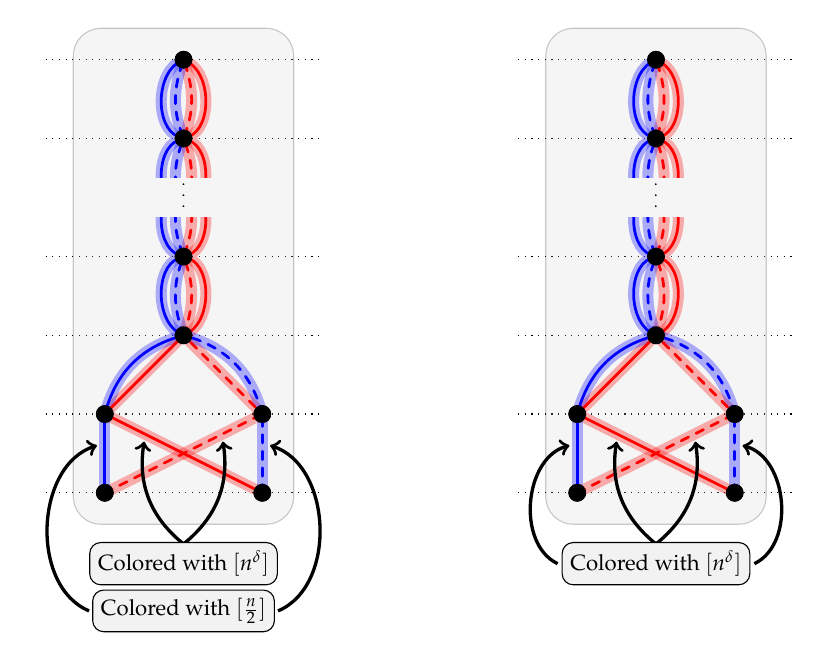
\begin{tikzpicture}
 
\begin{scope}[shift = {(4,0)}]

\draw[thin, dotted] (.25,0) to (3.75,0);
\draw[thin, dotted] (.25,1) to (3.75,1);
\draw[thin, dotted] (.25,2) to (3.75,2);
\draw[thin, dotted] (.25,3) to (3.75,3);
\draw[thin, dotted] (.25,4.5) to (3.75,4.5);
\draw[thin, dotted] (.25,5.5) to (3.75,5.5);

\draw[rounded corners = 10pt, fill = gray!40!, opacity =.2] (1-.4,5.5+.4) -- (3+.4,5.5+.4) -- (3+.4,0-.4) -- (1-.4,0-.4) -- cycle;

%%% RED %%%
\draw[rounded corners = 2pt, line width = 4pt, red, line cap = round, opacity = .3] (1,0) -- (3,1) -- (2,2);

\begin{scope}
\clip (1.5,2) rectangle (2.5,3.5);
\draw[rounded corners = 2pt, line width = 4pt, red, line cap = round, bend right = 20, opacity = .3] 
    (2,2) to (2,3) to (2,4);
\draw[rounded corners = 2pt, line width = 4pt, red, line cap = round, bend right = 70, opacity = .3] (2,2) to (2,3) to (2,4);
\end{scope}

\draw[rounded corners = 2pt, line width = 4pt, red, line cap = round, opacity = .3] (3,0) -- (1,1) -- (2,2);

%%% BLUE %%%
\draw[rounded corners = 2pt, line width = 4pt, blue, line cap = round, opacity = .3] (1,0) -- (1,1);
\draw[rounded corners = 2pt, line width = 4pt, blue, line cap = round, opacity = .3] (3,0) -- (3,1);

\begin{scope}
  \clip (1.5,2) rectangle (2.5,3.5);
\draw[rounded corners = 2pt, line width = 4pt, blue, line cap = round, bend left = 20, opacity = .3] (2,2) to (2,3) to (2,4);
\draw[rounded corners = 2pt, line width = 4pt, blue, line cap = round, bend left = 70, opacity = .3] (2,2) to (2,3) to (2,4);
\end{scope}

\draw[rounded corners = 2pt, line width = 4pt, blue, line cap = round, bend left = 30, opacity = .3] (1,1) to (2,2);
\draw[rounded corners = 2pt, line width = 4pt, blue, line cap = round, bend right = 30, opacity = .3] (3,1) to (2,2);

\begin{scope}
\clip (1.5,4) rectangle (2.5,5.5);
\draw[rounded corners = 2pt, line width = 4pt, red, line cap = round, bend right = 20, opacity = .3] 
    (2,3.5) to (2,4.5) to (2,5.5);
\draw[rounded corners = 2pt, line width = 4pt, red, line cap = round, bend right = 70, opacity = .3] (2,3.5) to (2,4.5) to (2,5.5);
\end{scope}

\begin{scope}
\clip (1.5,4) rectangle (2.5,5.5);
\draw[rounded corners = 2pt, line width = 4pt, blue, line cap = round, bend left = 20, opacity = .3] (2,3.5) to (2,4.5) to (2,5.5);
\draw[rounded corners = 2pt, line width = 4pt, blue, line cap = round, bend left = 70, opacity = .3] (2,3.5) to (2,4.5) to (2,5.5);
\end{scope}
           
\draw[fill = black] (1,0) circle (3pt);
\draw[fill = black] (3,0) circle (3pt);
\draw[fill = black] (1,1) circle (3pt);
\draw[fill = black] (3,1) circle (3pt);
\draw[fill = black] (2,2) circle (3pt);
\draw[fill = black] (2,3) circle (3pt);
\draw[fill = black] (2,4.5) circle (3pt);
\draw[fill = black] (2,5.5) circle (3pt);

\node at (2,3.875) {\tiny{$\vdots$}};
\end{scope}

%%%%%%%%%%%%%%% SECOND LINES %%%%%%%%%%%%%%%%%%%%%%%%%%%%%%%%

\begin{scope}[shift = {(4,0)}]
%%% RED %%%
\draw[rounded corners = 2pt, line width = 1pt, red, line cap = round, opacity = 1, dashed] (1,0) -- (3,1) -- (2,2);

\begin{scope}
\clip (1.5,2) rectangle (2.5,3.5);
\draw[rounded corners = 2pt, line width = 1pt, red, line cap = round, bend right = 20, opacity = 1, dashed] (2,2) to (2,3) to (2,4);
\draw[rounded corners = 2pt, line width = 1pt, red, line cap = round, bend right = 70, opacity = 1] (2,2) to (2,3) to (2,4);
\end{scope}

\draw[rounded corners = 2pt, line width = 1pt, red, line cap = round, opacity = 1] (3,0) -- (1,1) -- (2,2);

%%% BLUE %%%
\draw[rounded corners = 2pt, line width = 1pt, blue, line cap = round, opacity = 1] (1,0) -- (1,1);
\draw[rounded corners = 2pt, line width = 1pt, blue, line cap = round, opacity = 1, dashed] (3,0) -- (3,1);

\begin{scope}
 \clip (1.5,2) rectangle (2.5,3.5);
\draw[rounded corners = 2pt, line width = 1pt, blue, line cap = round, bend left = 20, opacity = 1, dashed] (2,2) to (2,3) to (2,4);
\draw[rounded corners = 2pt, line width = 1pt, blue, line cap = round, bend left = 70, opacity = 1] (2,2) to (2,3) to (2,4);
\end{scope}

\draw[rounded corners = 2pt, line width = 1pt, blue, line cap = round, bend left = 30, opacity = 1] (1,1) to (2,2);
\draw[rounded corners = 2pt, line width = 1pt, blue, line cap = round, bend right = 30, opacity = 1, dashed] (3,1) to (2,2);


\begin{scope}
 \clip (1.5,4) rectangle (2.5,5.5);
\draw[rounded corners = 2pt, line width = 1pt, red, line cap = round, bend right = 20, opacity = 1, dashed] (2,3.5) to (2,4.5) to (2,5.5);
\draw[rounded corners = 2pt, line width = 1pt, red, line cap = round, bend right = 70, opacity = 1] (2,3.5) to (2,4.5) to (2,5.5);
\end{scope}

\begin{scope}
\clip (1.5,4) rectangle (2.5,5.5);
\draw[rounded corners = 2pt, line width = 1pt, blue, line cap = round, bend left = 20, opacity = 1, dashed] (2,3.5) to (2,4.5) to (2,5.5);
\draw[rounded corners = 2pt, line width = 1pt, blue, line cap = round, bend left = 70, opacity = 1] (2,3.5) to (2,4.5) to (2,5.5);
\end{scope}
           
\draw[fill = black] (1,0) circle (3pt);
\draw[fill = black] (3,0) circle (3pt);
\draw[fill = black] (1,1) circle (3pt);
\draw[fill = black] (3,1) circle (3pt);
\draw[fill = black] (2,2) circle (3pt);
\draw[fill = black] (2,3) circle (3pt);
\draw[fill = black] (2,4.5) circle (3pt);
\draw[fill = black] (2,5.5) circle (3pt);

\node at (2,3.875) {\tiny{$\vdots$}};
\end{scope}



\begin{scope}[shift = {(4+6,0)}]

\draw[thin, dotted] (.25,0) to (3.75,0);
\draw[thin, dotted] (.25,1) to (3.75,1);
\draw[thin, dotted] (.25,2) to (3.75,2);
\draw[thin, dotted] (.25,3) to (3.75,3);
\draw[thin, dotted] (.25,4.5) to (3.75,4.5);
\draw[thin, dotted] (.25,5.5) to (3.75,5.5);

\draw[rounded corners = 10pt, fill = gray!40!, opacity =.2] (1-.4,5.5+.4) -- (3+.4,5.5+.4) -- (3+.4,0-.4) -- (1-.4,0-.4) -- cycle;

%%% RED %%%
\draw[rounded corners = 2pt, line width = 4pt, red, line cap = round, opacity = .3] (1,0) -- (3,1) -- (2,2);

\begin{scope}
\clip (1.5,2) rectangle (2.5,3.5);
\draw[rounded corners = 2pt, line width = 4pt, red, line cap = round, bend right = 20, opacity = .3] 
    (2,2) to (2,3) to (2,4);
\draw[rounded corners = 2pt, line width = 4pt, red, line cap = round, bend right = 70, opacity = .3] (2,2) to (2,3) to (2,4);
\end{scope}

\draw[rounded corners = 2pt, line width = 4pt, red, line cap = round, opacity = .3] (3,0) -- (1,1) -- (2,2);

%%% BLUE %%%
\draw[rounded corners = 2pt, line width = 4pt, blue, line cap = round, opacity = .3] (1,0) -- (1,1);
\draw[rounded corners = 2pt, line width = 4pt, blue, line cap = round, opacity = .3] (3,0) -- (3,1);

\begin{scope}
  \clip (1.5,2) rectangle (2.5,3.5);
\draw[rounded corners = 2pt, line width = 4pt, blue, line cap = round, bend left = 20, opacity = .3] (2,2) to (2,3) to (2,4);
\draw[rounded corners = 2pt, line width = 4pt, blue, line cap = round, bend left = 70, opacity = .3] (2,2) to (2,3) to (2,4);
\end{scope}

\draw[rounded corners = 2pt, line width = 4pt, blue, line cap = round, bend left = 30, opacity = .3] (1,1) to (2,2);
\draw[rounded corners = 2pt, line width = 4pt, blue, line cap = round, bend right = 30, opacity = .3] (3,1) to (2,2);

\begin{scope}
\clip (1.5,4) rectangle (2.5,5.5);
\draw[rounded corners = 2pt, line width = 4pt, red, line cap = round, bend right = 20, opacity = .3] 
    (2,3.5) to (2,4.5) to (2,5.5);
\draw[rounded corners = 2pt, line width = 4pt, red, line cap = round, bend right = 70, opacity = .3] (2,3.5) to (2,4.5) to (2,5.5);
\end{scope}

\begin{scope}
\clip (1.5,4) rectangle (2.5,5.5);
\draw[rounded corners = 2pt, line width = 4pt, blue, line cap = round, bend left = 20, opacity = .3] (2,3.5) to (2,4.5) to (2,5.5);
\draw[rounded corners = 2pt, line width = 4pt, blue, line cap = round, bend left = 70, opacity = .3] (2,3.5) to (2,4.5) to (2,5.5);
\end{scope}
           
\draw[fill = black] (1,0) circle (3pt);
\draw[fill = black] (3,0) circle (3pt);
\draw[fill = black] (1,1) circle (3pt);
\draw[fill = black] (3,1) circle (3pt);
\draw[fill = black] (2,2) circle (3pt);
\draw[fill = black] (2,3) circle (3pt);
\draw[fill = black] (2,4.5) circle (3pt);
\draw[fill = black] (2,5.5) circle (3pt);

\node at (2,3.875) {\tiny{$\vdots$}};
\end{scope}

%%%%%%%%%%%%%%% SECOND LINES %%%%%%%%%%%%%%%%%%%%%%%%%%%%%%%%

\begin{scope}[shift = {(4+6,0)}]
%%% RED %%%
\draw[rounded corners = 2pt, line width = 1pt, red, line cap = round, opacity = 1, dashed] (1,0) -- (3,1) -- (2,2);

\begin{scope}
\clip (1.5,2) rectangle (2.5,3.5);
\draw[rounded corners = 2pt, line width = 1pt, red, line cap = round, bend right = 20, opacity = 1, dashed] (2,2) to (2,3) to (2,4);
\draw[rounded corners = 2pt, line width = 1pt, red, line cap = round, bend right = 70, opacity = 1] (2,2) to (2,3) to (2,4);
\end{scope}

\draw[rounded corners = 2pt, line width = 1pt, red, line cap = round, opacity = 1] (3,0) -- (1,1) -- (2,2);

%%% BLUE %%%
\draw[rounded corners = 2pt, line width = 1pt, blue, line cap = round, opacity = 1] (1,0) -- (1,1);
\draw[rounded corners = 2pt, line width = 1pt, blue, line cap = round, opacity = 1, dashed] (3,0) -- (3,1);

\begin{scope}
 \clip (1.5,2) rectangle (2.5,3.5);
\draw[rounded corners = 2pt, line width = 1pt, blue, line cap = round, bend left = 20, opacity = 1, dashed] (2,2) to (2,3) to (2,4);
\draw[rounded corners = 2pt, line width = 1pt, blue, line cap = round, bend left = 70, opacity = 1] (2,2) to (2,3) to (2,4);
\end{scope}

\draw[rounded corners = 2pt, line width = 1pt, blue, line cap = round, bend left = 30, opacity = 1] (1,1) to (2,2);
\draw[rounded corners = 2pt, line width = 1pt, blue, line cap = round, bend right = 30, opacity = 1, dashed] (3,1) to (2,2);


\begin{scope}
 \clip (1.5,4) rectangle (2.5,5.5);
\draw[rounded corners = 2pt, line width = 1pt, red, line cap = round, bend right = 20, opacity = 1, dashed] (2,3.5) to (2,4.5) to (2,5.5);
\draw[rounded corners = 2pt, line width = 1pt, red, line cap = round, bend right = 70, opacity = 1] (2,3.5) to (2,4.5) to (2,5.5);
\end{scope}

\begin{scope}
\clip (1.5,4) rectangle (2.5,5.5);
\draw[rounded corners = 2pt, line width = 1pt, blue, line cap = round, bend left = 20, opacity = 1, dashed] (2,3.5) to (2,4.5) to (2,5.5);
\draw[rounded corners = 2pt, line width = 1pt, blue, line cap = round, bend left = 70, opacity = 1] (2,3.5) to (2,4.5) to (2,5.5);
\end{scope}
           
\draw[fill = black] (1,0) circle (3pt);
\draw[fill = black] (3,0) circle (3pt);
\draw[fill = black] (1,1) circle (3pt);
\draw[fill = black] (3,1) circle (3pt);
\draw[fill = black] (2,2) circle (3pt);
\draw[fill = black] (2,3) circle (3pt);
\draw[fill = black] (2,4.5) circle (3pt);
\draw[fill = black] (2,5.5) circle (3pt);

\node at (2,3.875) {\tiny{$\vdots$}};
\end{scope}


% 



\draw[very thick, ->, bend left = 30] (6,-.65) to (5.5,.65);
\draw[very thick, ->, bend right = 30] (6,-.65) to (6.5,.65);

\draw[very thick, ->, bend left = 70] (4.8,-1.5) to (4.9,.6);
\draw[very thick, ->, bend right = 70] (7.2,-1.5) to (7.1,.6);


\node[draw, fill=gray!10, rounded corners, inner sep=3pt] at (6,-.9) {\footnotesize{Colored with $[n^\delta]$}};


\node[draw, fill=gray!10, rounded corners, inner sep=3pt] at (6,-1.5) {\footnotesize{Colored with $[\frac{n}{2}]$}};

%%%%%

\draw[very thick, ->, bend left = 30] (6+6,-.65) to (5.5+6,.65);
\draw[very thick, ->, bend right = 30] (6+6,-.65) to (6.5+6,.65);

\draw[very thick, ->, bend left = 70] (4.75+6,-.9) to (4.9+6,.6);
\draw[very thick, ->, bend right = 70] (7.25+6,-.9) to (7.1+6,.6);

\node[draw, fill=gray!10, rounded corners, inner sep=3pt] at (6+6,-.9) {\footnotesize{Colored with $[n^\delta]$}};

\end{tikzpicture}
}

\item\adjustbox{valign=t}{
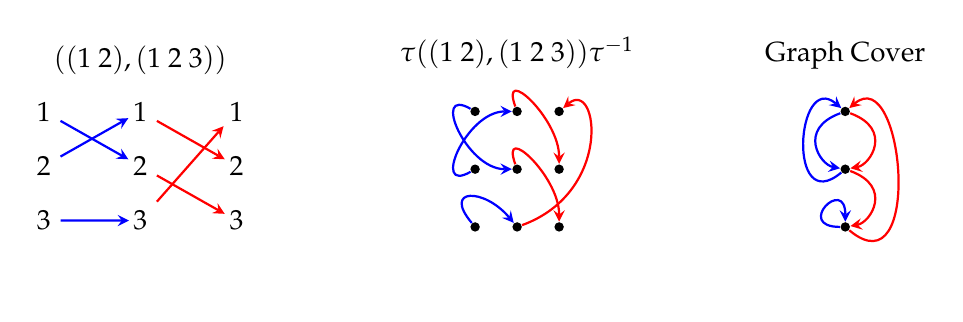
\begin{tikzpicture}[scale=.65,decoration={markings, mark=at position 0.55 with {\arrow[black]{stealth};}}]
    %%fig 1 labelled
     \node (a1) {1};
     \node (b1) [below=0.2cm of a1]{2};
     \node (c1) [below=0.2cm of b1]{3};
    
     \node (e1) [right=0.8cm of a1]{1};
     \node (f1) [right=0.8cm of b1]{2};
     \node (g1) [right=0.8cm of c1]{3};
    
     \node (i1) [right=0.8cm of e1]{1};
     \node (j1) [right=0.8cm of f1]{2};
     \node (k1) [right=0.8cm of g1]{3};
    
     \draw[thick, blue, -stealth, shorten >=-2pt] (a1) to node[auto] {} (f1);
     \draw[thick, blue, -stealth, shorten >=-2pt] (b1) to node[auto] {} (e1);
     \draw[thick, blue, -stealth, shorten >=-2pt] (c1) to node[auto] {} (g1);

     \draw[thick, red, -stealth, shorten >=-2pt] (e1) to node[auto] {} (j1);
     \draw[thick, red, -stealth, shorten >=-2pt] (f1) to node[auto] {} (k1);
     \draw[thick, red, -stealth, shorten >=-2pt] (g1) to node[auto] {} (i1);

    
     \node (d1) [right=0.2cm of a1]{};
     \node (d2) [right=0.2cm of e1]{};
     \node (s) [above=0.1cm of e1]{$((1 \ 2),(1 \ 2 \ 3))$};
    
    %% fig 2 unlabelled
     \node (a2)  [right=2.75cm of i1][fill,circle,inner sep=1.2pt] {};
     \node (b2) [below=0.6cm of a2][fill,circle,inner sep=1.2pt] {};
     \node (c2) [below=0.6cm of b2][fill,circle,inner sep=1.2pt] {};

    
     \node (e2) [right=0.4cm of a2][fill,circle,inner sep=1.2pt] {};
     \node (f2) [right=0.4cm of b2][fill,circle,inner sep=1.2pt] {};
     \node (g2) [right=0.4cm of c2][fill,circle,inner sep=1.2pt] {};

    
     \node (i2) [right=0.4cm of e2][fill,circle,inner sep=1.2pt] {};
     \node (j2) [right=0.4cm of f2][fill,circle,inner sep=1.2pt] {};
     \node (k2) [right=0.4cm of g2][fill,circle,inner sep=1.2pt] {};
     \node (t) [above=0.35cm of e2]{$\tau((1 \ 2),(1 \ 2 \ 3))\tau^{-1}$};
    
     \draw[thick, blue, -stealth] (a2) .. controls +(150:1) and +(180:1) .. (f2);
     \draw[thick, blue, -stealth] (b2) .. controls +(210:1) and +(180:1) .. (e2);
     \draw[thick, blue, -stealth] (c2)  .. controls +(130:1) and +(130:1) .. (g2);

     \draw[thick, red, -stealth] (e2) .. controls +(110:1) and +(90:1) .. (j2);
     \draw[thick, red, -stealth] (f2) .. controls +(110:1) and +(90:1) .. (k2);
     \draw[thick, red, -stealth] (g2).. controls +(20:2) and +(40:1) .. (i2);

    %% fig 3 unlabelled
     \node (a3) [right=3.5cm of i2][fill,circle,inner sep=1.2pt] {};
     \node (b3) [below=0.6cm of a3][fill,circle,inner sep=1.2pt] {};
     \node (c3) [below=0.6cm of b3][fill,circle,inner sep=1.2pt] {};
     \node (u) [above=0.35cm of a3]{Graph Cover};


     \draw[thick, blue, -stealth] (a3) .. controls +(200:1) and +(170:.5) .. (b3);
     \draw[thick, blue, -stealth] (b3) .. controls +(220:1.5) and +(140:1.25) .. (a3);
     \draw[thick, blue, -stealth] (c3)  .. controls +(180:1) and +(90:1) .. (c3);

     \draw[thick, red, -stealth] (a3) .. controls +(340:1) and +(10:0.5) .. (b3);
     \draw[thick, red, -stealth] (b3) .. controls +(340:1) and +(10:0.5) .. (c3);
     \draw[thick, red, -stealth] (c3).. controls +(320:2) and +(40:1.5) .. (a3);

    \end{tikzpicture}
}


\item\adjustbox{valign=t}{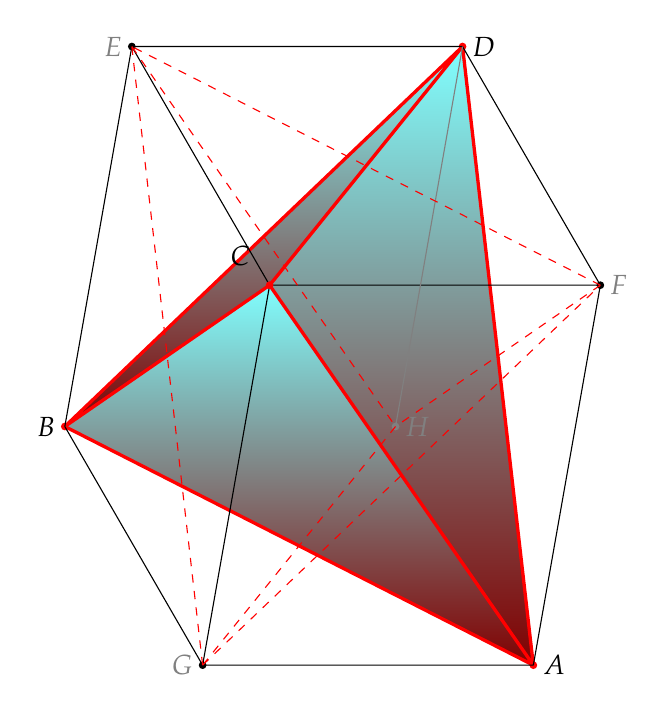
\begin{tikzpicture}[scale=0.7] 

% Figure parameters (tta and k needs to have the same sign)
% They can be modified at will
\def \tta{ -10.00000000000000 } % Defines the first angle of perspective
\def \k{    -3.00000000000000 } % Factor for second angle of perspective
\def \l{     6.00000000000000 } % Defines the width  of the parallelepiped
\def \d{     5.00000000000000 } % Defines the depth  of the parallelepiped
\def \h{     7.00000000000000 } % Defines the heigth of the parallelepiped

% The vertices A,B,C,D define the reference plan (vertical)
\coordinate (A) at (0,0); 
\coordinate (B) at ({-\h*sin(\tta)},{\h*cos(\tta)}); 
\coordinate (C) at ({-\h*sin(\tta)-\d*sin(\k*\tta)},
                    {\h*cos(\tta)+\d*cos(\k*\tta)}); 
\coordinate (D) at ({-\d*sin(\k*\tta)},{\d*cos(\k*\tta)}); 

% The vertices Ap,Bp,Cp,Dp define a plane translated from the 
% reference plane by the width of the parallelepiped
\coordinate (Ap) at (\l,0); 
\coordinate (Bp) at ({\l-\h*sin(\tta)},{\h*cos(\tta)}); 
\coordinate (Cp) at ({\l-\h*sin(\tta)-\d*sin(\k*\tta)},
                     {\h*cos(\tta)+\d*cos(\k*\tta)}); 
\coordinate (Dp) at ({\l-\d*sin(\k*\tta)},{\d*cos(\k*\tta)}); 

% Marking the vertices of the tetrahedron (red)
% and of the parallelepiped (black)
\fill[black]  (A) circle [radius=2pt]; 
\fill[red]    (B) circle [radius=2pt]; 
\fill[black]  (C) circle [radius=2pt]; 
\fill[red]    (D) circle [radius=2pt]; 
\fill[red]   (Ap) circle [radius=2pt]; 
\fill[black] (Bp) circle [radius=2pt]; 
\fill[red]   (Cp) circle [radius=2pt]; 
\fill[black] (Dp) circle [radius=2pt]; 

% painting first the three visible faces of the tetrahedron
\filldraw[draw=red,bottom color=red!50!black, top color=cyan!50]
  (B) -- (Cp) -- (D);
\filldraw[draw=red,bottom color=red!50!black, top color=cyan!50]
  (B) -- (D)  -- (Ap);
\filldraw[draw=red,bottom color=red!50!black, top color=cyan!50]
  (B) -- (Cp) -- (Ap);

% Draw the edges of the tetrahedron
\draw[red,-,very thick] (Ap) --  (D)
                        (Ap) --  (B)
                        (Ap) -- (Cp)
                        (B)  --  (D)
                        (Cp) --  (D)
                        (B)  -- (Cp);

% Draw the visible edges of the parallelepiped
\draw [-,thin] (B)  --  (A)
               (Ap) -- (Bp)
               (B)  --  (C)
               (D)  --  (C)
               (A)  --  (D)
               (Ap) --  (A)
               (Cp) --  (C)
               (Bp) --  (B)
               (Bp) -- (Cp);

% Draw the hidden edges of the parallelepiped
\draw [gray,-,thin] (Dp) -- (Cp);
                    (Dp) --  (D);
                    (Ap) -- (Dp);

% Name the vertices (the names are not consistent
%  with the node name, but it makes the programming easier)
\draw (Ap) node [right]           {$A$}
      (Bp) node [right, gray]     {$F$}
      (Cp) node [right]           {$D$}
      (C)  node [left,gray]       {$E$}
      (D)  node [left]            {$B$}
      (A)  node [left,gray]       {$G$}
      (B)  node [above left=+5pt] {$C$}
      (Dp) node [right,gray]      {$H$};

% Drawing again vertex $C$, node (B) because it disappeared behind the edges.
% Drawing again vertex $H$, node (Dp) because it disappeared behind the edges.
\fill[red]   (B) circle [radius=2pt]; 
\fill[gray] (Dp) circle [radius=2pt]; 

% From the reference and this example one can easily draw 
% the twin tetrahedron jointly to this one.
% Drawing the edges of the twin tetrahedron
% switching the p_s: A <-> Ap, etc...
\draw[red,-,dashed, thin] (A)  -- (Dp)
                          (A)  -- (Bp)
                          (A)  --  (C)
                          (Bp) -- (Dp)
                          (C)  -- (Dp)
                          (Bp) --  (C);
\end{tikzpicture}}

\item\adjustbox{valign=t}{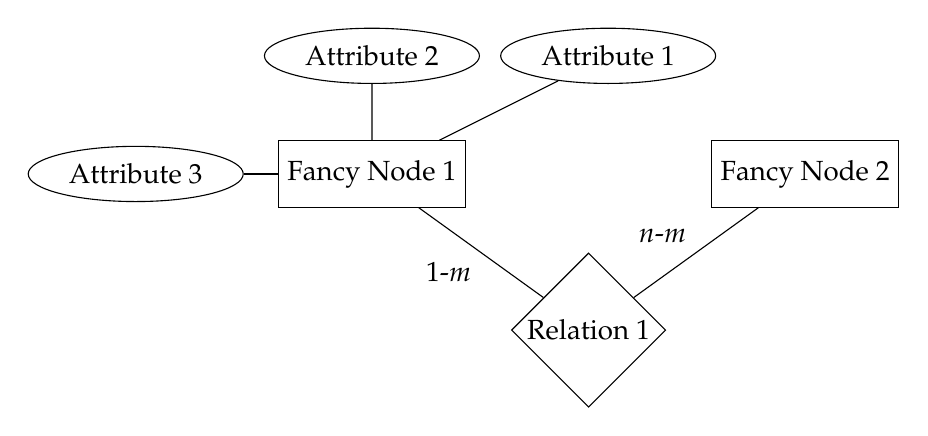
\begin{tikzpicture}[auto,node distance=1.5cm]
  % Create an entity with ID node1, label "Fancy Node 1".
  % Default for children (ie. attributes) is to be a tree "growing up"
  % and having a distance of 3cm.
  %
  % 2 of these attributes do so, the 3rd's positioning is overridden.
  \node[entity] (node1) {Fancy Node 1}
    [grow=up,sibling distance=3cm]
    child {node[attribute] {Attribute 1}}
    child {node[attribute] {Attribute 2}}
    child[grow=left,level distance=3cm] {node[attribute] {Attribute 3}};
  % Now place a relation (ID=rel1)
  \node[relationship] (rel1) [below right = of node1] {Relation 1};
  % Now the 2nd entity (ID=rel2)
  \node[entity] (node2) [above right = of rel1]	{Fancy Node 2};
  % Draw an edge between rel1 and node1; rel1 and node2
  \path (rel1) edge node {1-\(m\)} (node1)
    edge	 node {\(n\)-\(m\)}	(node2);
\end{tikzpicture}}





\item\adjustbox{valign=t}{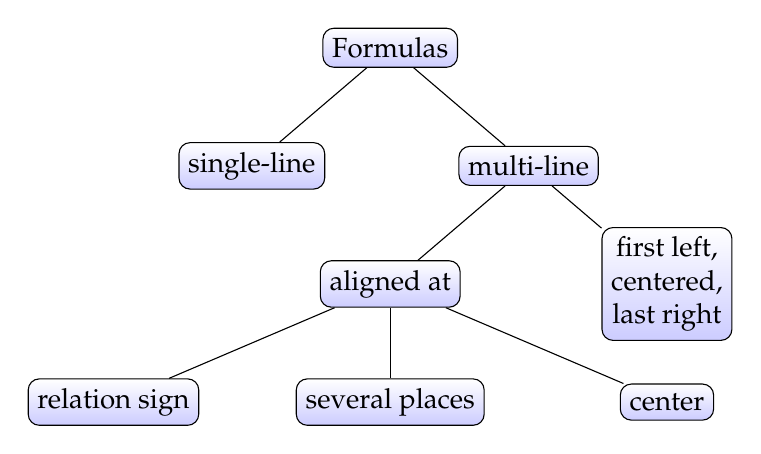
\begin{tikzpicture}[sibling distance=10em,
  every node/.style = {shape=rectangle, rounded corners,
    draw, align=center,
    top color=white, bottom color=blue!20}]]
  \node {Formulas}
    child { node {single-line} }
    child { node {multi-line}
      child { node {aligned at}
        child { node {relation sign} }
        child { node {several places} }
        child { node {center} } }
      child { node {first left,\\centered,\\last right} } };
\end{tikzpicture}}

\item \adjustbox{valign=t}{
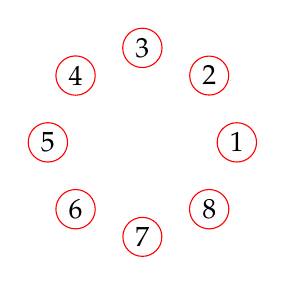
\begin{tikzpicture}
    \foreach \angle [count=\n] in {0,45,...,315}
    {\node[circle, draw=red,inner sep=2pt] at (\angle:1.2) {\n};
    }
\end{tikzpicture}
}




\end{enumerate}
\section{Geometry}

\begin{enumerate}



\item\adjustbox{valign=t}{
\begin{tikzpicture}
\draw (-2,0) -- (2,0);
\filldraw [gray] (0,0) circle (2pt);
\draw (-2,-2) .. controls (0,0) .. (2,-2);
\draw (-2,2) .. controls (-1,0) and (1,0) .. (2,2);
\end{tikzpicture}
}

\item\adjustbox{valign=t}{
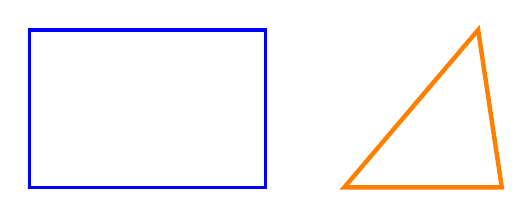
\begin{tikzpicture}
    \draw[blue, very thick] (0,0) rectangle (3,2);
\draw[orange, ultra thick] (4,0) -- (6,0) -- (5.7,2) -- cycle;
\end{tikzpicture}
}


\item\adjustbox{valign=t}{
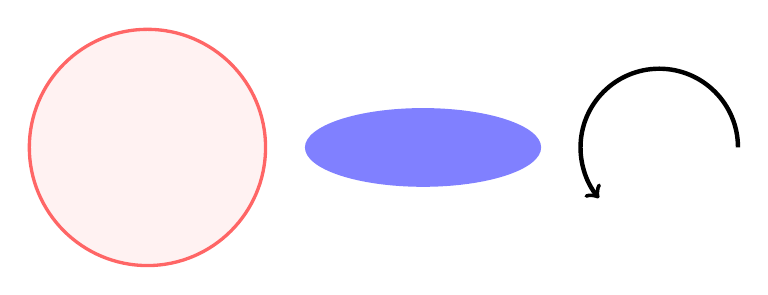
\begin{tikzpicture}
    \filldraw[color=red!60, fill=red!5, very thick](-1,0) circle (1.5);
\fill[blue!50] (2.5,0) ellipse (1.5 and 0.5);
\draw[ultra thick, ->] (6.5,0) arc (0:220:1);
\end{tikzpicture}

}




\item\adjustbox{valign=t}{
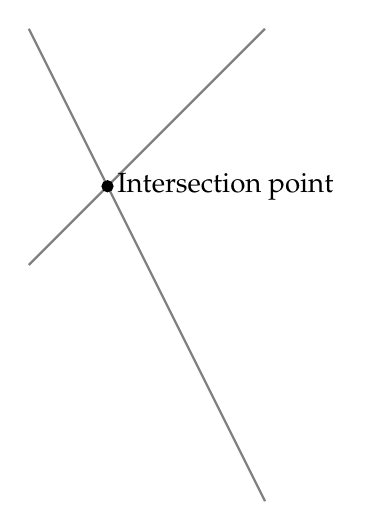
\begin{tikzpicture}
    \draw[gray, thick] (-1,2) -- (2,-4);
\draw[gray, thick] (-1,-1) -- (2,2);
\filldraw[black] (0,0) circle (2pt) node[anchor=west]{Intersection point};
\end{tikzpicture}
}

\item\adjustbox{valign=t}{
\newdimen\R
\R=0.8cm
\begin{tikzpicture}
    % Indicate the boundary of the regular polygons
    \draw [thin,black!20] circle (\R) ;
    \fill[black!20] circle (2pt);
    \draw (0:\R) \foreach \x in {120,240} {
            -- (\x:\R)
        } -- cycle (90:\R) node[above] {$n=3$} ;
    \draw[xshift=2.5\R] (0:\R) \foreach \x in {90,180,...,359} {
            -- (\x:\R)
        } -- cycle (90:\R) node[above] {$n=4$} ;
    \draw[xshift=5.0\R] (0:\R) \foreach \x in {72,144,...,359} {
            -- (\x:\R)
        } -- cycle (90:\R) node[above] {$n=5$} ;
    \begin{scope}[yshift=-3\R]
        \draw (0:\R) \foreach \x in {60,120,...,359} {
                -- (\x:\R)
            }-- cycle (90:\R) node[above] {$n=6$} ;
            
        % 360/7 = 51.4286 For PGF v < 1.18 we have to round to the nearest
        % integer. Newer version support fractional angle values.
        % For a more accurate result use the sequence
        % {51, 103, 154, 206, 257, 309}
        %
        \draw[xshift=2.5\R] (0:\R) \foreach \x in {51.4286,102.8571,...,359} {
                -- (\x:\R)
            }-- cycle (90:\R) node[above] {$n=7$} ;
        \draw[xshift=5.0\R] (0:\R) \foreach \x in {45,90,...,359} {
                -- (\x:\R)
            } -- cycle (90:\R) node[above] {$n=8$} ;
    \end{scope}
    \draw[yshift=-6.0\R] (0:\R) \foreach \x in {10,20,...,359} {
            -- (\x:\R)
        } -- cycle (90:\R) node[above] {$n=36$} ;
\end{tikzpicture}
}




    \item\adjustbox{valign=t}{
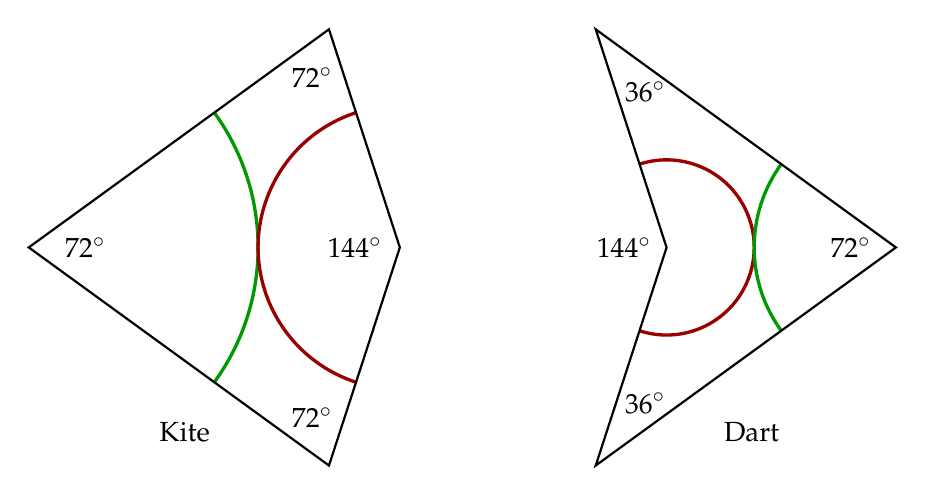
\begin{tikzpicture}[scale=1.8]

 \draw[very thick, green!60!black] (-36:1.618) arc (-36:36:1.618);
 \draw[very thick, red!60!black] ++(-36:2.618) ++(72:1.618) ++(108:1) arc (108:252:1);
 \draw[thick ] (0,0)--(-36:2.618)--++(72:1.618)--++(108:1.618)--cycle;
 \node  at (0.4,0) {$72^\circ$};
 \node  at (2.3,0) {$144^\circ$};
 \node  at (2,1.2) {$72^\circ$};
 \node  at (2,-1.2) {$72^\circ$};


 \node at (1.1,-1.3) {Kite};

 \begin{scope}[xshift=4.5cm]
 \draw[very thick, red!60!black] (-108:0.618) arc (-108:108:0.618);
 \draw[very thick, green!60!black] ++(108:1.618) ++(-36:1.618) arc (144:216:1);
 \draw[thick ] (0,0)--(108:1.618)--++(-36:2.618)--++(216:2.618)--cycle;
  \node  at (-0.3,0) {$144^\circ$};
 \node  at (1.3,0) {$72^\circ$};
 \node  at (-0.15,1.1) {$36^\circ$};
 \node  at (-0.15,-1.1) {$36^\circ$};

 \node at (0.6,-1.3) {Dart};
 \end{scope}
 
\end{tikzpicture}
}


\item\adjustbox{valign=t}{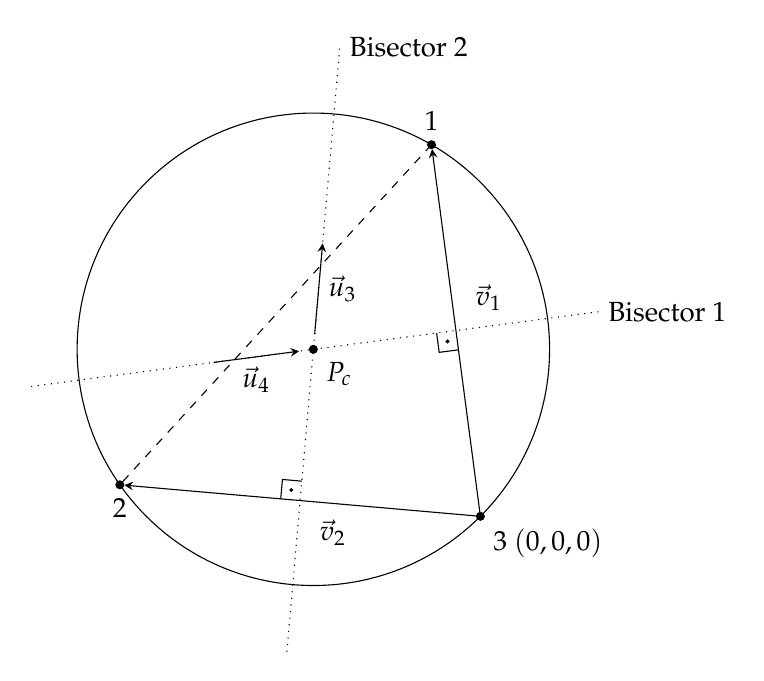
\begin{tikzpicture}
  [
    scale=3,
    >=stealth,
    point/.style = {draw, circle,  fill = black, inner sep = 1pt},
    dot/.style   = {draw, circle,  fill = black, inner sep = .2pt},
  ]

  % the circle
  \def\rad{1}
  \node (origin) at (0,0) [point, label = {below right:$P_c$}]{};
  \draw (origin) circle (\rad);

  % triangle nodes: just points on the circle
  \node (n1) at +(60:\rad) [point, label = above:$1$] {};
  \node (n2) at +(-145:\rad) [point, label = below:$2$] {};
  \node (n3) at +(-45:\rad) [point, label = {below right:$3$ $(0, 0, 0)$}] {};

  % triangle edges: connect the vertices, and leave a node at the midpoint
  \draw[->] (n3) -- node (a) [label = {above right:$\vec{v}_1$}] {} (n1);
  \draw[->] (n3) -- node (b) [label = {below right:$\vec{v}_2$}] {} (n2);
  \draw[dashed] (n2) -- (n1);

  % Bisectors
  % start at the point lying on the line from (origin) to (a), at
  % twice that distance, and then draw a path going to the point on
  % the line lying on the line from (a) to the (origin), at 3 times
  % that distance.
  \draw[dotted]
    ($ (origin) ! 2 ! (a) $)
    node [right] {Bisector 1}
    -- ($(a) ! 3 ! (origin)$ );

  % similarly for origin and b
  \draw[dotted]
    ($ (origin) ! 2 ! (b) $)
    -- ($(b) ! 3 ! (origin)$ )
    node [right] {Bisector 2};

  % short vectors
  \draw[->]
    ($ (origin) ! -.7 ! (a) $)
    -- node [below] {$\vec{u}_4$}
    ($ (origin) ! -.1 ! (a) $);
  \draw[->]
    ($ (origin) ! -.1 ! (b) $)
    -- node [right] {$\vec{u}_3$}
    ($ (origin) ! -.7 ! (b) $);

  % Right angle symbols
  \def\ralen{.5ex}  % length of the short segment
  \foreach \inter/\first/\last in {a/n3/origin, b/n2/origin}
    {
      \draw let \p1 = ($(\inter)!\ralen!(\first)$), % point along first path
                \p2 = ($(\inter)!\ralen!(\last)$),  % point along second path
                \p3 = ($(\p1)+(\p2)-(\inter)$)      % corner point
            in
              (\p1) -- (\p3) -- (\p2)               % path
              ($(\inter)!.5!(\p3)$) node [dot] {};  % center dot
    }
\end{tikzpicture}}



\item\adjustbox{valign=t}{\begin{tikzpicture}
  \coordinate [label={below right:$A$}] (A) at (0, 0);
  \coordinate [label={above right:$B$}] (B) at (0, \pythagheight);
  \coordinate [label={below left:$C$}] (C) at (-\pythagwidth, 0);

  \coordinate (D1) at (-\pythagheight, \pythagheight + \pythagwidth);
  \coordinate (D2) at (-\pythagheight - \pythagwidth, \pythagwidth);

  \draw [very thick] (A) -- (C) -- (B) -- (A);

  \newcommand{\ranglesize}{0.3cm}
  \draw (A) -- ++ (0, \ranglesize) -- ++ (-\ranglesize, 0) -- ++ (0, -\ranglesize);

  \draw [dashed] (A) -- node [below] {$b$} ++ (-\pythagwidth, 0)
            -- node [right] {$b$} ++ (0, -\pythagwidth)
            -- node [above] {$b$} ++ (\pythagwidth, 0)
            -- node [left]  {$b$} ++ (0, \pythagwidth);

  \draw [dashed] (A) -- node [right] {$c$} ++ (0, \pythagheight)
            -- node [below] {$c$} ++ (\pythagheight, 0)
            -- node [left]  {$c$} ++ (0, -\pythagheight)
            -- node [above] {$c$} ++ (-\pythagheight, 0);

  \draw [dashed] (C) -- node [above left]  {$a$} (B)
                     -- node [below left]  {$a$} (D1)
                     -- node [below right] {$a$} (D2)
                     -- node [above right] {$a$} (C);
\end{tikzpicture}}





\item\adjustbox{valign=t}{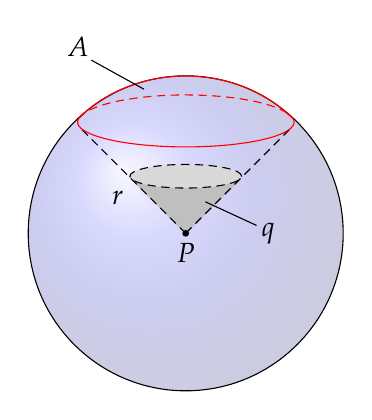
\begin{tikzpicture}
  \coordinate (O) at (0,0);

  % ball background color
  \shade[ball color = blue, opacity = 0.2] (0,0) circle [radius = 2cm];

  % cone
  \begin{scope}
    \def\rx{0.71}% horizontal radius of the ellipse
    \def\ry{0.15}% vertical radius of the ellipse
    \def\z{0.725}% distance from center of ellipse to origin

    \path [name path = ellipse]    (0,\z) ellipse ({\rx} and {\ry});
    \path [name path = horizontal] (-\rx,\z-\ry*\ry/\z)
                                -- (\rx,\z-\ry*\ry/\z);
    \path [name intersections = {of = ellipse and horizontal}];

    % radius to base of cone in ball
    \draw[fill = gray!50, gray!50] (intersection-1) -- (0,0)
      -- (intersection-2) -- cycle;
    % base of cone in ball
    \draw[fill = gray!30, densely dashed] (0,\z) ellipse ({\rx} and {\ry});
  \end{scope}

  % label of cone
  \draw (0.25,0.4) -- (0.9,0.1) node at (1.05,0.0) {$q$};

  % ball
  \draw (O) circle [radius=2cm];
  % label of ball center point
  \filldraw (O) circle (1pt) node[below] {$P$};

  % radius
  \draw[densely dashed] (O) to [edge label = $r$] (-1.33,1.33);
  \draw[densely dashed] (O) -- (1.33,1.33);

  % cut of ball surface
  \draw[red] (-1.35,1.47) arc [start angle = 140, end angle = 40,
    x radius = 17.6mm, y radius = 14.75mm];
  \draw[red, densely dashed] (-1.36,1.46) arc [start angle = 170, end angle = 10,
    x radius = 13.8mm, y radius = 3.6mm];
  \draw[red] (-1.29,1.52) arc [start angle=-200, end angle = 20,
    x radius = 13.75mm, y radius = 3.15mm];

  % label of cut of ball surface
  \draw (-1.2,2.2) -- (-0.53,1.83) node at (-1.37,2.37) {$A$};
\end{tikzpicture}}


\end{enumerate}
\section{Games}

\begin{enumerate}
    \item\adjustbox{valign=t}{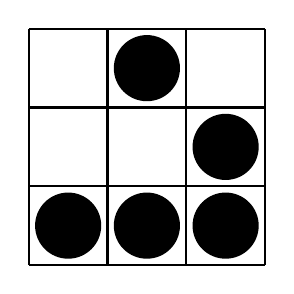
\begin{tikzpicture}[thick]
\draw (0,0) grid (3,3);
\foreach \c in {(0,0), (1,0), (2,0), (2,1), (1,2)}
    \fill \c + (0.5,0.5) circle (0.42);
\end{tikzpicture}}





\item\adjustbox{valign=t}{
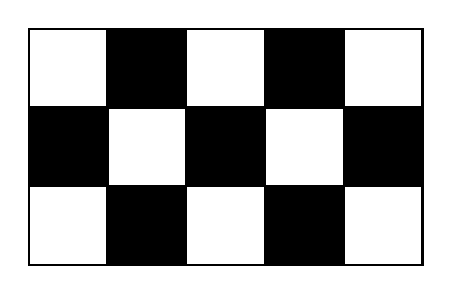
\begin{tikzpicture}
\foreach \r in {0 ,1 ,2} {
\foreach \c in {0 ,1 ,...,4} {
\pgfmathsetmacro \n {\r +\c }
\ifodd \n
\draw [ thick , fill = black ] (\c -1 ,\r -1) rectangle (\c ,\r ); \else
\draw [ thick , fill = white ] (\c -1 ,\r -1) rectangle (\c ,\r ); 
\fi
}
}
\end{tikzpicture}
}



\item\adjustbox{valign=t}{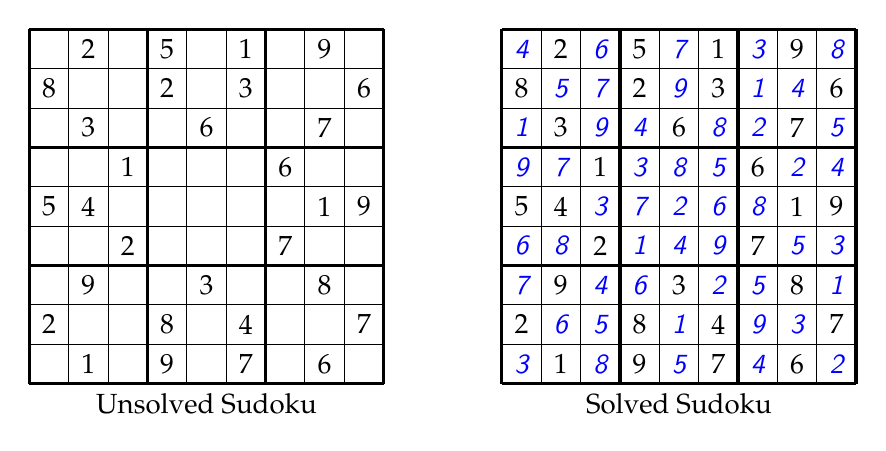
\begin{tikzpicture}[scale=.5]

  \begin{scope}
    \draw (0, 0) grid (9, 9);
    \draw[very thick, scale=3] (0, 0) grid (3, 3);

    \setcounter{row}{1}
    \setrow { }{2}{ }  {5}{ }{1}  { }{9}{ }
    \setrow {8}{ }{ }  {2}{ }{3}  { }{ }{6}
    \setrow { }{3}{ }  { }{6}{ }  { }{7}{ }

    \setrow { }{ }{1}  { }{ }{ }  {6}{ }{ }
    \setrow {5}{4}{ }  { }{ }{ }  { }{1}{9}
    \setrow { }{ }{2}  { }{ }{ }  {7}{ }{ }

    \setrow { }{9}{ }  { }{3}{ }  { }{8}{ }
    \setrow {2}{ }{ }  {8}{ }{4}  { }{ }{7}
    \setrow { }{1}{ }  {9}{ }{7}  { }{6}{ }

    \node[anchor=center] at (4.5, -0.5) {Unsolved Sudoku};
  \end{scope}

  \begin{scope}[xshift=12cm]
    \draw (0, 0) grid (9, 9);
    \draw[very thick, scale=3] (0, 0) grid (3, 3);

    \setcounter{row}{1}
    \setrow { }{2}{ }  {5}{ }{1}  { }{9}{ }
    \setrow {8}{ }{ }  {2}{ }{3}  { }{ }{6}
    \setrow { }{3}{ }  { }{6}{ }  { }{7}{ }

    \setrow { }{ }{1}  { }{ }{ }  {6}{ }{ }
    \setrow {5}{4}{ }  { }{ }{ }  { }{1}{9}
    \setrow { }{ }{2}  { }{ }{ }  {7}{ }{ }

    \setrow { }{9}{ }  { }{3}{ }  { }{8}{ }
    \setrow {2}{ }{ }  {8}{ }{4}  { }{ }{7}
    \setrow { }{1}{ }  {9}{ }{7}  { }{6}{ }

    \node[anchor=center] at (4.5, -0.5) {Solved Sudoku};

    \begin{scope}[blue, font=\sffamily\slshape]
      \setcounter{row}{1}
      \setrow {4}{ }{6}  { }{7}{ }  {3}{ }{8}
      \setrow { }{5}{7}  { }{9}{ }  {1}{4}{ }
      \setrow {1}{ }{9}  {4}{ }{8}  {2}{ }{5}

      \setrow {9}{7}{ }  {3}{8}{5}  { }{2}{4}
      \setrow { }{ }{3}  {7}{2}{6}  {8}{ }{ }
      \setrow {6}{8}{ }  {1}{4}{9}  { }{5}{3}

      \setrow {7}{ }{4}  {6}{ }{2}  {5}{ }{1}
      \setrow { }{6}{5}  { }{1}{ }  {9}{3}{ }
      \setrow {3}{ }{8}  { }{5}{ }  {4}{ }{2}
    \end{scope}

  \end{scope}

\end{tikzpicture}}


\end{enumerate}






\section{Data}

\begin{enumerate}
    \item\adjustbox{valign=t}{
\begin{tikzpicture}
\begin{axis}
\addplot[color=red]{exp(x)};
\end{axis}
\end{tikzpicture}
%Here ends the 2D plot
\hskip 5pt
%Here begins the 3D plot
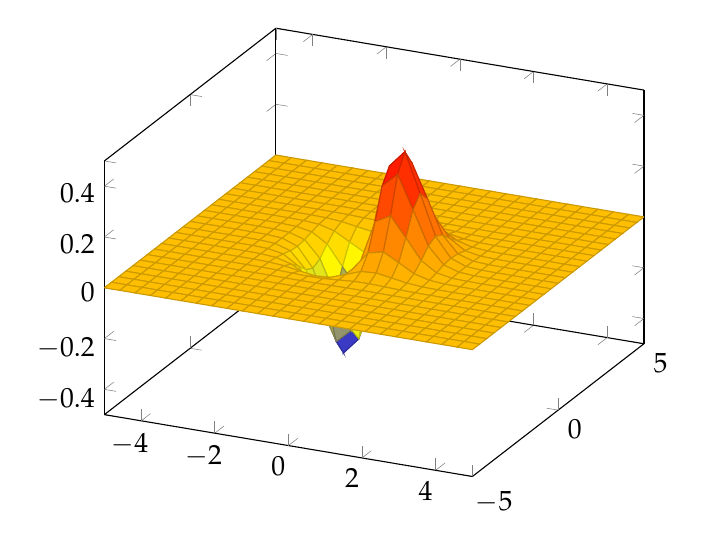
\begin{tikzpicture}
\begin{axis}
\addplot3[
    surf,
]
{exp(-x^2-y^2)*x};
\end{axis}
\end{tikzpicture}
%Here ends the 3D plot
}





\item\adjustbox{valign=t}{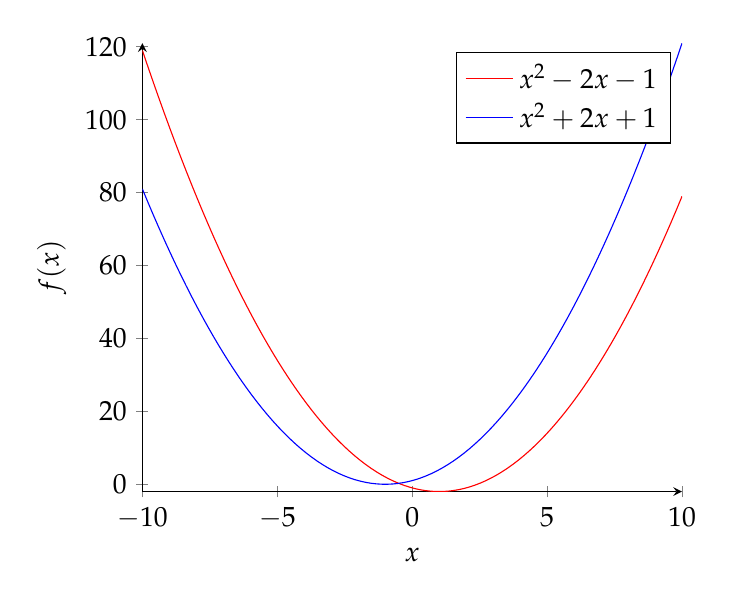
\begin{tikzpicture}
\begin{axis}[
    axis lines = left,
    xlabel = \(x\),
    ylabel = {\(f(x)\)},
]
%Below the red parabola is defined
\addplot [
    domain=-10:10, 
    samples=100, 
    color=red,
]
{x^2 - 2*x - 1};
\addlegendentry{\(x^2 - 2x - 1\)}
%Here the blue parabola is defined
\addplot [
    domain=-10:10, 
    samples=100, 
    color=blue,
    ]
    {x^2 + 2*x + 1};
\addlegendentry{\(x^2 + 2x + 1\)}

\end{axis}
\end{tikzpicture}}




\item\adjustbox{valign=t}{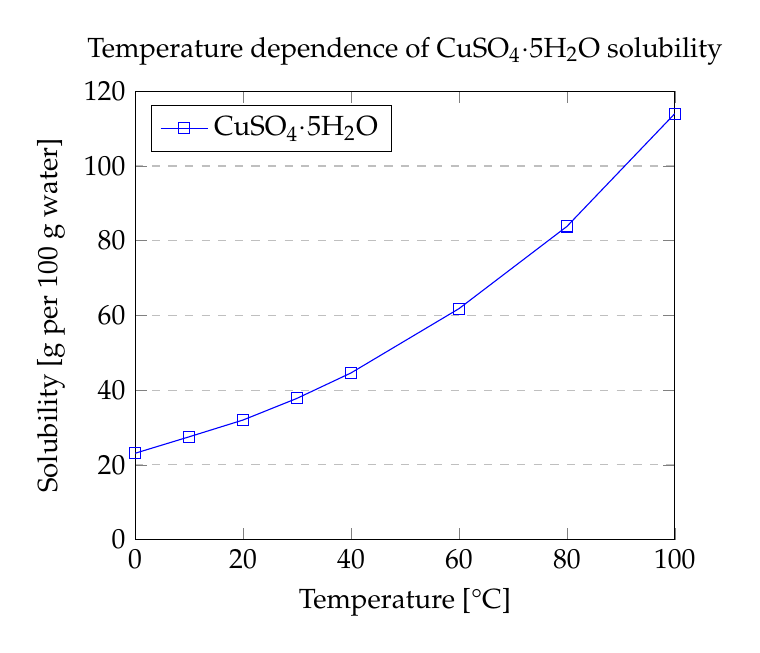
\begin{tikzpicture}
\begin{axis}[
    title={Temperature dependence of CuSO\(_4\cdot\)5H\(_2\)O solubility},
    xlabel={Temperature [\textcelsius]},
    ylabel={Solubility [g per 100 g water]},
    xmin=0, xmax=100,
    ymin=0, ymax=120,
    xtick={0,20,40,60,80,100},
    ytick={0,20,40,60,80,100,120},
    legend pos=north west,
    ymajorgrids=true,
    grid style=dashed,
]

\addplot[
    color=blue,
    mark=square,
    ]
    coordinates {
    (0,23.1)(10,27.5)(20,32)(30,37.8)(40,44.6)(60,61.8)(80,83.8)(100,114)
    };
    \legend{CuSO\(_4\cdot\)5H\(_2\)O}
    
\end{axis}
\end{tikzpicture}}




\item\adjustbox{valign=t}{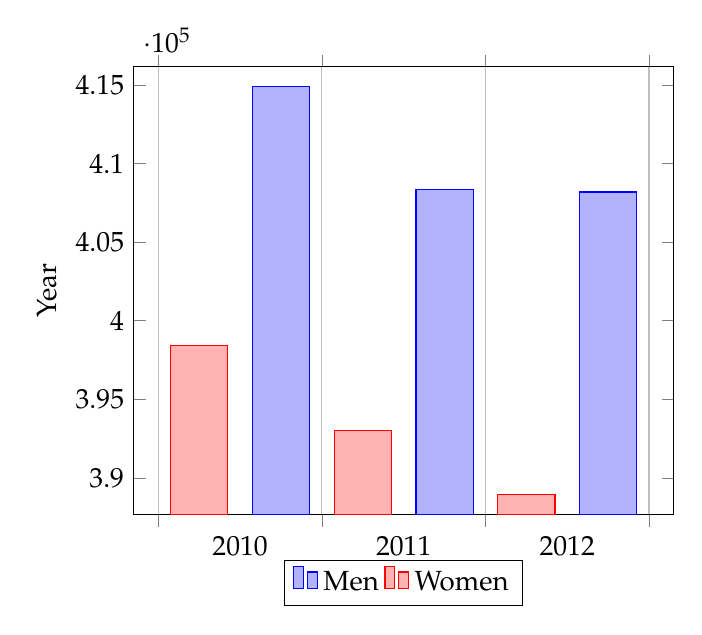
\begin{tikzpicture}
\begin{axis}[
	x tick label style={
		/pgf/number format/1000 sep=},
	ylabel=Year,
	enlargelimits=0.05,
	legend style={at={(0.5,-0.1)},
	anchor=north,legend columns=-1},
	ybar interval=0.7,
]
\addplot 
	coordinates {(2012,408184) (2011,408348)
		 (2010,414870) (2009,412156)};
\addplot 
	coordinates {(2012,388950) (2011,393007) 
		(2010,398449) (2009,395972)};
\legend{Men,Women}
\end{axis}
\end{tikzpicture}}




\item\adjustbox{valign=t}{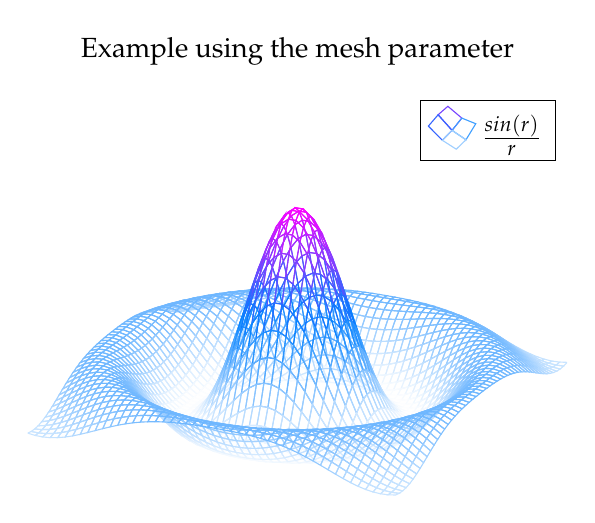
\begin{tikzpicture}
\begin{axis}[
    title=Example using the mesh parameter,
    hide axis,
    colormap/cool,
]
\addplot3[
    mesh,
    samples=50,
    domain=-8:8,
]
{sin(deg(sqrt(x^2+y^2)))/sqrt(x^2+y^2)};
\addlegendentry{\(\frac{sin(r)}{r}\)}
\end{axis}
\end{tikzpicture}}





\item\adjustbox{valign=t}{\begin{tikzpicture}
\begin{axis}
[
    title={Contour plot, view from top},
    view={0}{90}
]
\addplot3[
    contour gnuplot={levels={0.8, 0.4, 0.2, -0.2}}
]
{sin(deg(sqrt(x^2+y^2)))/sqrt(x^2+y^2)};
\end{axis}
\end{tikzpicture}}


\item\adjustbox{valign=t}{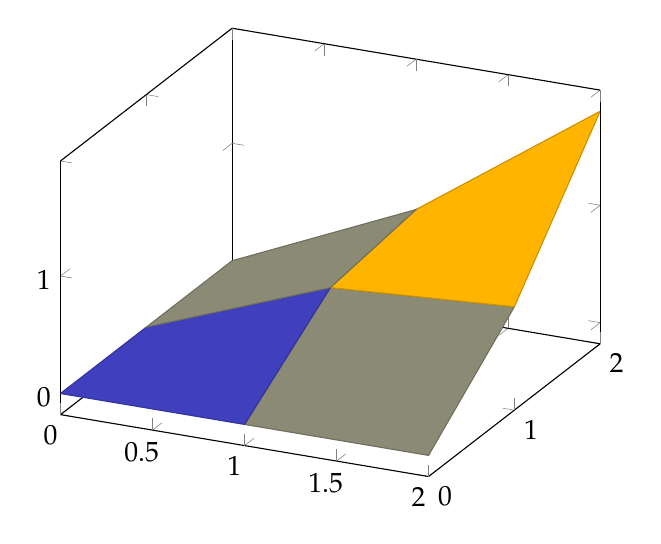
\begin{tikzpicture}
\begin{axis}
\addplot3[
    surf,
] 
coordinates {
(0,0,0) (0,1,0) (0,2,0)

(1,0,0) (1,1,0.6) (1,2,0.7)

(2,0,0) (2,1,0.7) (2,2,1.8)
};
\end{axis}
\end{tikzpicture}}



\item\adjustbox{valign=t}{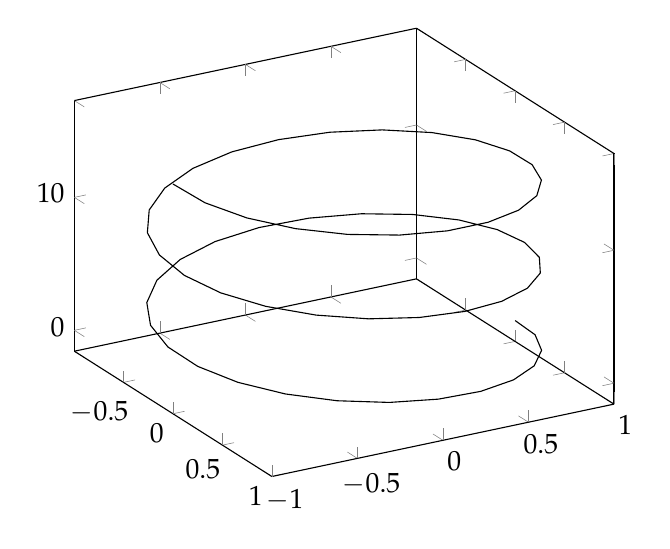
\begin{tikzpicture}
\begin{axis}
    [
    view={60}{30},
    ]
\addplot3[
    domain=0:5*pi,
    samples = 60,
    samples y=0,
]
({sin(deg(x))},
{cos(deg(x))},
{x});
\end{axis}
\end{tikzpicture}}



\end{enumerate}
\section{Miscellaneous}

\begin{enumerate}
   \item\adjustbox{valign=t}{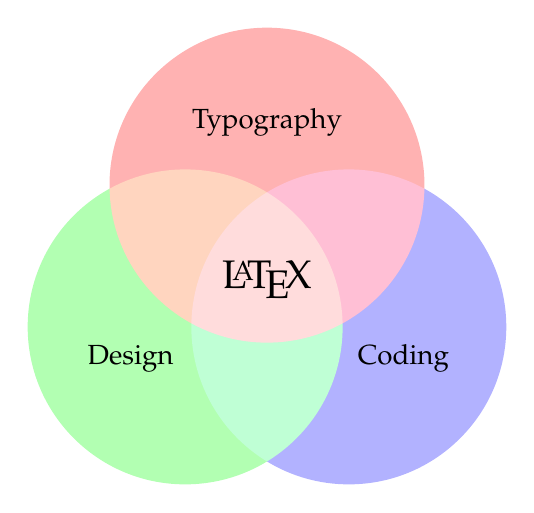
\begin{tikzpicture}
  \begin{scope}[blend group = soft light]
    \fill[red!30!white]   ( 90:1.2) circle (2);
    \fill[green!30!white] (210:1.2) circle (2);
    \fill[blue!30!white]  (330:1.2) circle (2);
  \end{scope}
  \node at ( 90:2)    {Typography};
  \node at ( 210:2)   {Design};
  \node at ( 330:2)   {Coding};
  \node [font=\Large] {\LaTeX};
\end{tikzpicture}}
\end{enumerate}



















%\item \adjustbox{valign=t}{\begin{tikzpicture}[scale=0.5]
  % Label
 % \node[right] at (-5,4) {\small $y = x^5$};

  % Axes
 % \draw[latex-latex, very thick] (-5.3,0)--(5.3,0);
  %\draw[latex-latex, very thick] (0,-5.3)--(0,5.3);

  % Graph
 % \begin{scope}
  %  \clip(-5,-5) rectangle (5,5);
 %   \draw[domain=-1.5:1.5, smooth, variable=\x, black, samples=120, very thick] plot ({\x},{(\x)^5});
  %\end{scope}
%\end{tikzpicture}}









\end{document}